% This is the HU Berlin LaTeX template, optimized for R Markdown.

% -------------------------------
% --- PREAMBLE ---
% -------------------------------
\documentclass[a4paper,11pt]{article}

\usepackage{amsmath,amssymb,amsfonts,amsthm}    % Typical maths resource packages
\usepackage{graphicx}                           % Packages to allow inclusion of graphics
\usepackage{tabularx}
\usepackage[authoryear]{natbib}                 % literature reference style
\usepackage[utf8]{inputenc}


\usepackage[margin=10pt,font=small,labelfont=bf,
labelsep=endash]{caption}

\usepackage{textcomp}                           % For single quotes
\usepackage{floatrow}                           % For image and table position
\usepackage{booktabs}                           % For tables
% \usepackage[colorlinks=true]{hyperref}                           
% \usepackage[bottom]{footmisc}                   
\usepackage[bottom, flushmargin]{footmisc}                   % For footnotes
\usepackage[citebordercolor={0 1 0}]{hyperref}                           % For creating hyperlinks in cross references
\usepackage{footnotebackref}

% -------------------------------
% --- some layout definitions ---
% -------------------------------

% define topline
\usepackage[automark]{scrlayer-scrpage}
\pagestyle{scrheadings}
\automark{section}
\clearscrheadings
\ohead{\headmark}

% define citation style
\bibliographystyle{abbrvnat}

% define page size, margin size
\setlength{\headheight}{1.1\baselineskip}
\voffset=-2cm
\hoffset=-3cm
\textheight24cm
\textwidth15.5cm
\topmargin1cm
\oddsidemargin3cm
\evensidemargin3cm
\setcounter{secnumdepth}{3}
\setcounter{tocdepth}{3}   
  \usepackage[parfill]{parskip} 

% define line spacing = 1.5
\renewcommand{\baselinestretch}{1.1}

% define position of graphics
\floatsetup[figure]{capposition=bottom}
\floatsetup[table]{capposition=bottom}
\floatplacement{figure}{ht}
\floatplacement{table}{ht}

% save thesis parameters for later
\newcommand{\thesistype}{Master's Thesis}
\newcommand{\thesisauthor}{Harm van Kuppevelt}
\newcommand{\thesisdate}{August, 2021}

% define tightlist to work with newer versions of pandoc
\providecommand{\tightlist}{%
  \setlength{\itemsep}{0pt}\setlength{\parskip}{0pt}}


\newlength{\cslhangindent}
\setlength{\cslhangindent}{1.5em}
\newenvironment{CSLReferences}%
  {}%
  {\par}

% change spacing
\setlength {\parskip}{1em}

% Additional LaTeX parameters added in the YAML header of index.Rmd



% --------------------------------------
% --------------------------------------
% --------------------------------------
% --- the structure the tex document ---
% ---  (this our recommendation) -------
% frontmatter:
%   - titlepage (mandatory),
%   - acknowledgement,
%   - abstract,
%   - table of contents (mandatory),
%   - list of abbreviations (not mandatory),
%   - list of figures (not mandatory),
%   - list of tables  (not mandatory) .
%
% body of the thesis (the structure of the thesis body is not mandatory, but the list of literature is mandatory):
%   - introduction,
%   - methods,
%   - data,
%   - results,
%   - conclusion,
%   - literature (mandatory),
%   - appendix (figures, tables).
%
% last page:
%   - declaration of authorship (mandatory).
% --------------------------------------
% --------------------------------------
% --------------------------------------
\begin{document}
% -------------------------------
% --- frontmatter: Title page ---
% -------------------------------
\thispagestyle{empty}
\begin{center}
  {\Large{\bf Addition of iron (oxy)hydroxides to ditches in a peat meadow reduces the internal phosphorus loading}} \vspace{0.5cm}

  Master's Thesis submitted \\\vspace{0.5cm}
  to \\\vspace{0.5cm}
  \textbf{Dr.~Thilo Behrends} \\
  \textbf{Melanie Münch Msc.} \\\vspace{0.5cm}
  Utrecht University \\
  Faculty of Geosciences \\
  Department of Earth sciences \\
   Geochemistry \\  \vspace{1cm}

  
\includegraphics[width=0.5\textwidth]{UU_logo_EN_CMYK.png}
  
  by \\\vspace{0.5cm}
  \textbf{Harm van Kuppevelt} \\
  (4061985) \\
  
  \medskip
  \medskip
  in partial fulfillment of the requirements \\
  for the degree of \\
  \textbf{Master of Earth Science} \\\vspace{0.5cm}
  August, 2021
  
\end{center}
% ------------------------------------
% --- frontmatter: Acknowledgement ---
% ------------------------------------
\newpage
\hypertarget{acknowledgements}{%
\section*{Acknowledgements}\label{acknowledgements}}
\addcontentsline{toc}{section}{Acknowledgements}

First and foremost I want to thank my supervisors Thilo Behrends and Melanie Münch, for sharing their knowledge and practical help, and I especially enjoyed the fruitful discussions. I also want to thank all PhD and master students I have had the honor to meet during the practical work, for the lively conversations we had during breaks and outside of university.
\pagestyle{plain}
\pagenumbering{roman}   % define page number in roman style
\setcounter{page}{1}    % start page numbering

% -----------------------------
% --- frontmatter: Abstract ---
% -----------------------------
\newpage
\hypertarget{abstract}{%
\section*{Abstract}\label{abstract}}
\addcontentsline{toc}{section}{Abstract}

Ecological damage by phosphate (P) pollution in aquatic environments is a growing problem. Legacy P released from sediments impedes the restoration of water quality of freshwater systems even with no external influx of P. The internal P loading causes prolonged eutrophication which in turn causes anoxia and very harmful for aquatic organisms. Internal P loading can persist for a very long time, so for restoration purposes it is necessary to mitigate internal loading effectively. A promising method is the fixation of P in the sediment with iron (Fe) compounds. In this study, we investigate the ditch system in Bovenlanden, a wet peat meadow in the Western peat area in the Netherlands. In two ditches of the system, iron-containing by-products from drinking water treatment, predominately consisting of iron (oxy)hydroxides, have been added six months before in order to mitigate internal P loading. Here, we evaluate the effect of Fe treatment on the P and Fe dynamics and composition of the sediment, and on the benthic fluxes of P and Fe. We used a sequential extraction procedure to identify iron speciation in the sediment and examine P associated with Fe phases. Benthic fluxes were monitored under laboratory conditions in sediment cores from treated and non-treated ditches in the area, under both oxic and anoxic conditions. We found Fe concentrations up to an order of magnitude larger in the treated sediment compared to untreated sediment. The Fe in the treated sediment was mainly extracted by HCl. Most P was extracted by HCl as well, in both treated and untreated cores. Coinciding with elevated solid Fe content, Fe concentrations in the porewater of the treated cores were high, ranging from 30\(\mu\)M up to 350 \(\mu\)M. In contrast, P concentrations were lowered significantly (\textless{} 5 \(\mu\)M) at depth intervals with high Fe contents, compared to the high P concentrations in the non-treated cores (5-100 \(\mu\)M). The difference in dissolved P and Fe in the porewater was reflected by the benthic flux results, where P fluxes have decreased an order of magnitude as result of Fe treatment. This shows that within the timescale of this study, the treatment of peaty ditches with Fe-containing by-products is an effective way to suppress internal P loading.

% -----------------------------
% --- frontmatter: Contents ---
% -----------------------------
\newpage
\tableofcontents
\clearpage

% ----------------------------------------------------------
% --- frontmatter: List of Abbreviations (not mandatory) ---
% ----------------------------------------------------------

% ----------------------------------------------------
% --- frontmatter: List of Figures (not mandatory) ---
% ----------------------------------------------------

% ---------------------------------------------------
% --- frontmatter: List of Tables (not mandatory) ---
% ---------------------------------------------------

% -------------------------------
% --- main body of the thesis ---
% -------------------------------
\newpage
\pagestyle{plain}       
\setcounter{page}{1}    % start page numbering anew
\pagenumbering{arabic}  % page numbers in arabic style

\hypertarget{introduction}{%
\section{Introduction}\label{introduction}}

Since the the invention of agriculture, humanity has had influence on Earths natural cycles, and this increased dramatically after the start of the industrial revolution. One of these profound impacts, and most damaging for freshwater ecosystems has been a large increase in available phosphorous (P) dissolved the surface water. P, on earth predominantly found in oxidized form as phosphate (PO\(_4^{3-}\)), is crucial for many biochemical processes, and typically a limiting nutrient for plant growth as natural release from minerals is a relatively slow process. (\protect\hyperlink{ref-schindlerFoodWebStructure1993}{D. E. Schindler et al. 1993}) For this reason, P availability has been an constraint for food production during most of human history, when agriculture could only be sustained on fertile soil where P was replenished, such as floodplains, and P-rich manure was a valuable commodity. (\protect\hyperlink{ref-ashleyBriefHistoryPhosphorus2011}{Ashley, Cordell, and Mavinic 2011}) From the 19th century onwards people have turned to mineral sources of P in an effort to feed the growing human population. At first, guano (accumulated bird droppings), became the primary source material for fertilizers, but as guano reserves became increasingly scarce, the large scale mining of rocks rich in P took over. In combination with artificially fixated nitrogen, mined P forms the bulk of all fertilizers used today, and without a continued P supply we would not be able to produce enough food to sustain the current population. (\protect\hyperlink{ref-cordell2010}{Cordell 2010}; \protect\hyperlink{ref-vaccariDemandDrivenModelGlobal2019}{Vaccari, Powers, and Liu 2019}) However, the intensive use of mineral P has disrupted the natural P cycle, and replaced it with a linear lifecycle, where a finite supply of P rock provides the P for plant growth, while the P containing products are shipped globally and accumulates elsewhere, ultimately ending up in oceans lakes and soils.(\protect\hyperlink{ref-ashleyBriefHistoryPhosphorus2011}{Ashley, Cordell, and Mavinic 2011}) This linear P pathway is not only threatening food security in the future when mineral P reserves will ultimately deplete, today already we encounter severe problems caused by P accumulation. (\protect\hyperlink{ref-ansariEutrophicationCausesConsequences2011}{Ansari et al. 2011}; \protect\hyperlink{ref-mekonnenGlobalAnthropogenicPhosphorus2018}{Mekonnen and Hoekstra 2018})

\hypertarget{the-problem-with-p-eutrophication}{%
\subsection{The problem with P: eutrophication}\label{the-problem-with-p-eutrophication}}

The increased concentration of P in fresh surface waters disrupt the nutrient balance on which the ecosystem has relied before, where P is a limiting nutrient. (\protect\hyperlink{ref-schindlerFoodWebStructure1993}{D. E. Schindler et al. 1993}) Not constrained by P scarcity, autotrophic microorganisms can multiply exponentially in number. The enrichment of water bodies with high amounts of nutrients and following phytoplankton bloom is called eutrophication. (\protect\hyperlink{ref-ansariEutrophicationCausesConsequences2011}{Ansari et al. 2011}) The algae or cyanobecteria blooms block incoming radiation, hindering plant growth. The loss of aquatic plants, combined with an increase in decaying organic matter (OM) from dead plants and detritus, create very low redox conditions above the sediment, resulting in anoxia. (\protect\hyperlink{ref-correllRolePhosphorusEutrophication1998}{Correll 1998}) The lack of oxygen leads to loss of aerobic respirators, including aquatic animals, and this further increases the stockpile of dead OM, enhancing the reductive conditions. (\protect\hyperlink{ref-matthewsLongTermChanges2006}{Matthews and Effler 2006}) In addition to suppressed oxygen availability, eutrophication causes ecological damage when the anoxic conditions allow harmful substances to release from the sediment, notably sulfide (HS\(^-\)) and ammonium (NH\(_4^+\)), both toxic for aquatic life in high concentrations. Meanwhile, P levels remain high through reduction of metal oxides adsorbing P, together with P release from organic matter mineralization.

\hypertarget{external-and-internal-loading}{%
\subsection{External and internal loading}\label{external-and-internal-loading}}

Eutrophication rarely develops in natural systems, only where the small natural P fluxes can accumulate over time, and develops on geological timescales. (\protect\hyperlink{ref-ansariEutrophicationCausesConsequences2014}{Ansari and Gill 2014}) It is therefore primarily a phenomenon caused by human activities, and is more widespread than it would be under natural circumstances.

The increase in P concentaration starts when P rich water enters the lake or river. This external source of P is commonly referred to as external P loading. Raw sewage and wastewater have polluted waters near urban centers since before industrialization and the issue persists today in many parts of the world. (\protect\hyperlink{ref-ashleyBriefHistoryPhosphorus2011}{Ashley, Cordell, and Mavinic 2011}; \protect\hyperlink{ref-azamPhosphorousEnvironmentCharacteristics2019}{Azam et al. 2019}) Due to improvements in wastewater treatment, the external P load in Europe was reduced and P levels in European rivers and lakes have on avarage decreased since 1992. (\protect\hyperlink{ref-NutrientsFreshwaterEurope}{{``Nutrients in Freshwater in {Europe} {} {European Environment Agency},''} n.d.}) However, the average P concentration has stabilized in recent years at still dangerously high levels, as P load from agricultural runoff has become a major pollutant, and causes widespread eutrophication many areas. (\protect\hyperlink{ref-ansariEutrophicationCausesConsequences2011}{Ansari et al. 2011}; \protect\hyperlink{ref-mekonnenGlobalAnthropogenicPhosphorus2018}{Mekonnen and Hoekstra 2018}) The large global increase in demand for animal products such as meat and dairy provoked an upscale and intensification of livestock farming, leading to vast numbers of production animals kept close together. Via imported animal feed, the nutrients from large sections of farmland are thus concentrated within a small area, and often leak to the local surface water. It is for this reason that almost all freshwater systems in areas with large-scale intensive livestock farming, such as the Netherlands, experience some degree of eutrophication. (\protect\hyperlink{ref-mekonnenGlobalAnthropogenicPhosphorus2018}{Mekonnen and Hoekstra 2018})
\begin{figure}

{\centering 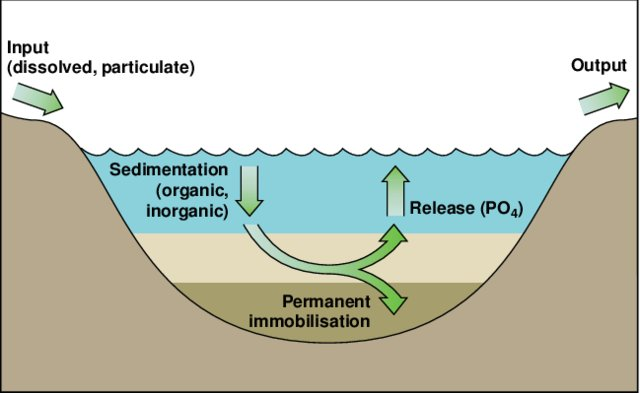
\includegraphics[width=0.75\linewidth]{C:/Users/harmv/Documents/studie/scriptie/Master/Master_Thesis/index/figures/load} 

}

\caption{Cycling of  P in lakes: External and internal P loading. P deposited in the lake sediment over time is released again.}\label{fig:intern}
\end{figure}
From research on lake restoration during the 20th century it became clear that eutrophication persists even if all external sources are removed, as the source of P lies within the lake sediment itself, hence: internal P loading.\protect\hyperlink{ref-schindlerRecentAdvancesUnderstanding2006}{D. W. Schindler} (\protect\hyperlink{ref-schindlerRecentAdvancesUnderstanding2006}{2006}) The recycling of P is a natural process OM containing P settles on the lake sediment, and P is released when OM mineralizes in the sediment (Fig. \ref{fig:intern}). The P cycling is thus closely linked to the cycling of OM in lakes, which depends on primary production. In eutrophic systems, primary production is high, thus OM and P are deposited at an increased rate. When a freshwater system has experienced eutrophication from external sources over a long period of time, much of the P is sequestered in the sediment by OM deposition. (\protect\hyperlink{ref-oconnellChangesSedimentaryPhosphorus2020}{D. O'Connell et al. 2020}) After the removal of an external source, decomposing OM releases P to the water column, and this recycling of P can keep the water eutrophic for decades after external loading has been removed. (\protect\hyperlink{ref-chorusDecadesNeededEcosystem2020}{Chorus et al. 2020}; \protect\hyperlink{ref-sondergaardRetentionInternalLoading2001}{Søndergaard, Jensen, and Jeppesen 2001})

\hypertarget{lake-restoration-targeting-internal-p-loading}{%
\subsection{Lake restoration targeting internal P loading}\label{lake-restoration-targeting-internal-p-loading}}

The extent of the ecological damage from eutrophication prompted efforts to restore water quality of lakes and rivers in some places. However, eliminating external loading, by insulating the system from nutrient rich water sources in the vicinity and allowing only small-scale agriculture nearby, is often not sufficient, particularly if the system has been severely eutrophic for a long time. For healthy P levels, the internal P loading has to be lowered as well. Physical removing the sediment by dredging will remove some of the P rich layer, but is an expensive method and is not always effective as it is restricted in how much sediment can be removed, and high P concentrations often persist deep in the sediment. (\protect\hyperlink{ref-zamparasRestorationEutrophicFreshwater2014}{Zamparas and Zacharias 2014}) Moreover, it is an invasive technique which disturbs the sediment and risks contaminating the water. The problem of internal loading stems from the high dissolved fraction of P in the sediment, so a promising solution is to bind the P in the sediment so release is stopped. (\protect\hyperlink{ref-azamPhosphorousEnvironmentCharacteristics2019}{Azam et al. 2019}) Several materials are used as a P-sorption agent in other applications and could be used to mitigate internal P loading, including modified zeolites, lanthanum enhanced clays and aluminum compounds. (\protect\hyperlink{ref-azamPhosphorousEnvironmentCharacteristics2019}{Azam et al. 2019}) While some of the materials have a high adsorption capacity for P, a lot has to be added to effectively bind the large reservoir of P in the sediment, which can be an expensive endeavor. Moreover, the solids could be buried deeper while phosphate rich sediment remains close to the surface, making this method less effective. Iron (Fe) compounds are particularly of interest for P binding in sediment. While less absorptive compared to materials designed to bind P such as lanthanum clays, Fe is abundantly available and can easily applied in large quantities.

\hypertarget{issues-of-using-fe-to-bind-p}{%
\subsection{Issues of using Fe to bind P}\label{issues-of-using-fe-to-bind-p}}

In contrast to most sorbents used to bind P, Fe is relatively reactive, and sensitive to redox conditions. While this is problematic for some applications, the redox sensitivity of iron can be an advantage for containing P in the sediment. Fe is found in many natural systems, and the redox-driven cycling in lake sediments is well documented. (\protect\hyperlink{ref-emersonEarlyDiagenesisAnaerobic1976}{Emerson 1976}) Solid phase ferric iron (Fe\(^{3+}\)) in sediments with low redox conditions can be used by chemotrophs as electron acceptor and reduced to ferrous iron (Fe\(^{2+}\)) which is generally more soluble. The now mobile Fe\(^{2+}\) can diffuse back to the surface, where it is oxidized again and precipitates in the form of iron oxides. The reductive dissolution of Fe was previously thought to lower its effectiveness as sorbent, as less adsorption sites remain available. However, through this process Fe is continue recycled and remains close to the surface where it can adsorb P released in the sediment. (\protect\hyperlink{ref-kleebergHowEffectivelyDoes2012}{Kleeberg, Köhler, and Hupfer 2012}) This so called ``ferrous wheel'' forms in this way an quasi-permanent layer of iron oxides on top, which is an effective trap for P in the sediment. This mechanism can remain in effect until the Fe pool is saturated with P (Fig. \ref{fig:fwheel}). Ideally, the P is bound deeper in the sediment as well to Fe\(^{2+}\) to form vivianite (Fe\(_3\)(PO\(_4\))\(_2\))), removing the P from the system entirely. (\protect\hyperlink{ref-emersonEarlyDiagenesisAnaerobic1976}{Emerson 1976}; \protect\hyperlink{ref-rotheOccurrenceIdentificationEnvironmental2016}{Matthias Rothe, Kleeberg, and Hupfer 2016})
\begin{figure}

{\centering 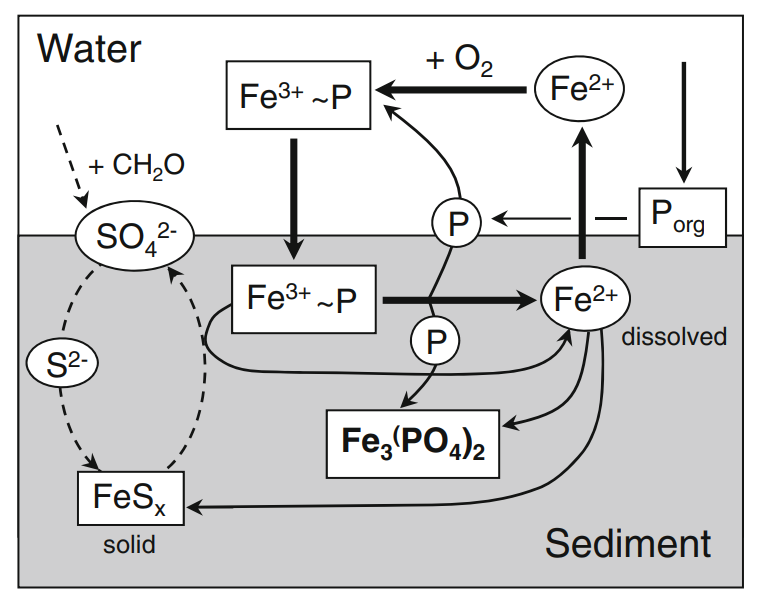
\includegraphics[width=0.8\linewidth]{C:/Users/harmv/Documents/studie/scriptie/Master/Master_Thesis/index/figures/ferrouswheel} 

}

\caption{Simple schematic representation of the ferrous wheel controlling the P dynamics in the sediment. Fe oxides with P adsorbed dissolves through reduction in the sediment. The now mobilized ferrous iron dffuses to the water column, where it is oxidized again and precipititates together with phosphate, thus forming a cycle. In this figure possibility of forming vivianite (Fe$_3$(PO$_4$)$_2$) is also presented. Fe is removed from the ferrous wheel when it reacts with dissolved sulfide, and precipitates. Figure modefied from  Kleeberg et al. (2012).}\label{fig:fwheel}
\end{figure}
\hypertarget{fe-containing-by-products}{%
\subsection{Fe containing by-products}\label{fe-containing-by-products}}

Fe can be added to the system in several forms: as salt, or directly as solid oxide. At Bovenlanden, the research site of this study, Fe-containing by-products from water treatment was used to treat several ditches with the goal of reducing internal P loading. Water from subsurface aquifers contains substantial concentrations of Fe, and to make the water potable Fe is precipitated through aeration and filtered. The precipitate which is the by-product consists primarily of ferric (oxyhydr)oxides. Many water treatment plants produce the by-product and it is therefore available in large volumes at low costs.

\hypertarget{peat-wetlands-in-the-netherlands-and-their-restoration}{%
\subsection{Peat wetlands in the Netherlands and their restoration}\label{peat-wetlands-in-the-netherlands-and-their-restoration}}

As part of the Rhine delta, marine clay deposition and peat layers formed the Western part of the Netherlands during the Holocene. Originally comprised of mainly inhabitable peat bogs and tidal marches, the area was drained and cultivated gradually during medieval times. A system of ditches, canals and lakes developed as a result of drainage practices, and the intensive extraction of peat as energy source. (\protect\hyperlink{ref-borgerDrainingDiggingDredging1992}{Borger 1992}) In an effort to stimulate dairy production, intense farming of cattle was introduced in the area during the 20th century. As a consequence, most surface water is highly increased in nutrients, and eutrophication is widespread. In recent years the negative effects of land reclamation and intensive agriculture of peat marches has attracted more attention. Dry peat soils cause subsidence and emit significant amounts of carbon dioxide. Efforts to re-wet parts of the western peat area are combined with restoration goals for biodiversity, as many meadow birds characteristic for this kind of landscape can thrive on wet grassland. However, the plentiful lakes and ditches in the area remain polluted by nutrients. (\protect\hyperlink{ref-keizerPhosphorusSedimentLoosdrecht1992}{Keizer and Sinke 1992}) Improvement of surface water quality is essential to restore the nutrient poor conditions of biodiverse types farmland common in this area before the industrial revolution.

\hypertarget{objectives}{%
\subsection{objectives}\label{objectives}}

Treating freshwater systems with iron has been done before, and it has been shown that many parameters control the cycling of P and Fe. Several studies have shown that high sulfur (S) content can weaken the effectiveness of Fe treatment by binding the iron as sulfide. \protect\hyperlink{ref-smoldersSulphatemediatedIronLimitation1993}{Smolders and Roelofs} (\protect\hyperlink{ref-smoldersSulphatemediatedIronLimitation1993}{1993}) Other studies show that OM is important in the cycling of P and Fe. (\protect\hyperlink{ref-oconnellChangesSedimentaryPhosphorus2020}{D. O'Connell et al. 2020}; \protect\hyperlink{ref-schwertmannNatureIronOxide1988}{Schwertmann and Murad 1988}) As hydrological and geochemical conditions vary widely between systems, its effect on P and Fe dynamics is uncertain. The ditches in Bovenlanden were treated to mitigate internal P loading, but the resulting sediment composition nor the biogeochemical cycling of P and Fe has been investigated. In this study, we will do this by comparing the sediment of a treated ditch in Bovenlanden to sediment from untreated ditches in the same area.
By analyzing samples from the field in detail and monitoring the nutrient dynamics under laboratory conditions, we aim to answer the following questions:
\begin{itemize}
\item
  Can the Fe from treatment be recognized in the sediment, and what is the Fe speciation?
\item
  Did iron treatment bind P in the sediment, and in which binding form?
\item
  How does iron treatment influence the internal P load in peat extraction ditches?
\end{itemize}
\hypertarget{methodology}{%
\section{Methodology}\label{methodology}}

\hypertarget{study-site}{%
\subsection{Study site}\label{study-site}}

Sediment cores and surface water were gathered at Bovenlanden, a peat meadow in South-Holland, the Netherlands (N 52°, 9' E 4°,52'). (Fig. \ref{fig:BL}) The area functioned as farmland in the past, and is heavily influenced by fertilization. Nowdays, Bovenlanden is managed by Natuurmonumenten, in a conservation effort to restore biodiversity in the western peat meadow system of the Netherlands. The goal is to restore types of grassland common before industrialization of farming, which have typically more diverse vegetation and form a habitat for breeding meadow birds. To establish a nutrient poor wet meadow, water quality had to be improved. To reduce external influx of P, most ditches in the southern part have been detached from the surrounding surface water, keeping only one inlet via a weir, and runoff from land was reduced by removing the top layer of soil containing most of the nutrients. In 2020, 60 tons of iron sludge was added to the southern two ditches to mitigate internal P loading. Water quality improved on visual inspection after a few months after the treatment.
\begin{figure}

{\centering \includegraphics[width=1\linewidth]{C:/Users/harmv/Documents/studie/scriptie/Master/Master_Thesis/index/figures/BovenlandenOverview} 

}

\caption{Overview of the study site. On the left  the general location within the Netherlands is shown. In the bottom right is indicated where Bovenlanden is located within the western peat area. On the right a satelite image of Bovenlanden with important features highlighted. Two ditches in the area have been treated with iron sludge in the past. Note the only water inlet is located in the north, far away from the treated ditches}\label{fig:BL}
\end{figure}
\hypertarget{core-sampling}{%
\subsection{Core sampling}\label{core-sampling}}

Sediment cores were collected on site the 23rd of February 2021. Two locations on the same treated ditch were chosen based on distance from the inlet weir, each treated location was paired with a reference location in a non-treated ditch nearby. (Fig. \ref{fig:sampleloc}) For each of the four locations 7 cores were collected using a UWITEC corer with a diameter of 6 cm. Sediment depth in the cores was approximately 40 cm, with 20cm overlying water. Extra surface water was collected for refilling during incubation sampling. Temperature, pH, dissolved oxygen, and electrical conductivity were measured using probes. Surface water samples were collected and filtered on site using 0.45\(\mu\)m pore size nylon syringe filters. 10 mL was subsampled for Fe and P measurement, and directly acidified with 1\% 3.75M HNO\(_3\), and another 2mL subsampled and treated by adding 0.2\% zinc acetate to fix sulfide. All surface water samples and subsamples were stored cool.
\begin{figure}

{\centering \includegraphics[width=1\linewidth]{C:/Users/harmv/Documents/studie/scriptie/Master/Master_Thesis/index/figures/BovenlandenSampleLocations} 

}

\caption{Four location within the Bovenlanden system where samples have been taken. On the northern of the two treated ditches, two locations on opposide sides were chosen: A and C. To differentiate from the non-treated locations, they are displayed in red. Two nearby locations in untreated ditches, B and D, are displayed in blue. The two sides of the ditch were chosen to investigate the possible influence of surface water influx, as locations B and D are closer to the water inlet in the north of the system. }\label{fig:sampleloc}
\end{figure}
Directly after the field campaign, one core from each location was sliced for porewater and sediment analysis. Slicing was performed under low oxygen conditions in a glovebag filled with nitrogen gas. Slices were removed with a plastic spoon at intervals of 1cm for the top 10cm, and 2cm intervals at greater depth. Sediment slices were collected in 50mL centrifuge tubes and centrifuged at 3000rpm for 10min to separate porewater from the solid sediment. In a glovebox with nitrogen atmosphere, the porewater was decanted into a syringe with a 0.45\(\mu\)m nylon filter and filtered into four subsamples: 5mL acidified with 1\% 3.75M HNO\(_3\) for Fe and P measurements, 2mL with 0.2\% zinc acetate for sulfide measurement, 1mL in a vial for ion chromatography, and the remainder for measuring ammonium. The solid sediment was freezedried, and homogenized with an agate mortal and pestle under nitrogen atmosphere. Wet samples were stored cool (5°C) in airtight containers, dry sediment was kept under nitrogen atmosphere.

\hypertarget{sequential-extractions-of-fe-pools}{%
\subsection{Sequential extractions of Fe pools}\label{sequential-extractions-of-fe-pools}}

Analysis of the iron pools in the solid phase was done with a sequential extraction method based on \protect\hyperlink{ref-claffSequentialExtractionProcedure2010}{Claff et al.} (\protect\hyperlink{ref-claffSequentialExtractionProcedure2010}{2010}). The method was modified to include phosphate measurements of the extracted pools by omitting the pyrophosphate extraction in the main sequential extraction. Relatively low concentrations of phosphate in the extract is not distinguishable from pyrophosphate using elemental analysis, and a test confirmed that photometric phosphate analysis did not work in a pyrophosphate matrix. Furthermore, the chemical similarity between pyrophosphate and phosphate could influence the phosphate binding to iron in other phases other than the targeted organic bound iron. For this reason, a two-step extraction of MgCl and pyrophosphate was performed parallel to the main extraction to target iron complexed with organic matter. (Table \ref{tab:seqextr})

Approximately 100mg of dry sediment was weighed into a 15mL centrifuge tube. For each extraction step, 10 mL of extraction solution was added with a dispenser under a continuous nitrogen flow. After addition, the mixture was weighed, resuspended and shaken for a specified time. After extraction, the suspension was centrifuged for 10min at 3000rpm, and the supernatant decanted into a syringe with 0.45\(\mu\)m filter and the next extraction solution was added immediately. The extractant was filtered and diluted 10 times before analysis (see below). The last extraction step, which uses concentrated nitric acid and therefore very reactive to material left in the filter, was not filtered and diluted 100 times to bring to a workable pH.
\begin{table}[ht]
 \centering
     {\footnotesize
        \begin{tabular}{m{0.1\textwidth} m{0.07\textwidth} | m{0.1\textwidth} m{0.3\textwidth} m{0.1\textwidth} m{0.2\textwidth}}
            \hline \hline
                  & step  & name & extractant & extraction time & target pool      \\
            \hline
                Extraction A   & 1 & MgCl & 1M magnesium chloride solution & 1h & exchangeable iron, iron salts \\
                   & 2 & HCl & 1M hydochloric acid & 4h & easily dissolving iron oxides and sulfides, carbonates\\
                   & 3 & CBD & 50 g/l sodium dithionite in 0.35 M acetic acid and 0.2 M sodium citrate buffer (pH 4.8)  & 4h & crystalline iron oxides \\
                   & 4 & HNO$_3$ & concentrated nitric acid (67\%)& 2h & pyrite\\
                   \hline
                    Extraction B   & 1 & MgCl$_2$ & 1M magnesium chloride solution & 1h & exchangeable iron, iron salts\\
                    & 2 & pyrophosphate & 0.1M sodium pyrophosphate solution & 16h & organic complexed iron\\
            \hline \hline
        \end{tabular}}
    \caption{Sequential extraction procedure for determining Fe speciation. The extraction is performed in multiple steps using different solvents to extract iron phases. The sequence is build up so each step targets a subsequent pool with lower reactivity. The procedure is modefied from Claff (2010) by removing the organic targeting pyrophosphate extraction from the sequence and instead to perform a parallel pyrophosphate extraction, here listed as extraction B.  }
    \label{tab:seqextr}
    \end{table}
\hypertarget{incubation-setup-for-benthic-flux-measurements}{%
\subsection{Incubation setup for benthic flux measurements}\label{incubation-setup-for-benthic-flux-measurements}}

To monitor benthic fluxes under oxic and anoxic conditions, sediment cores where incubated in a climate chamber at 10°C for 60 days. For each location two cores were allowed to turn anoxic, and two where kept oxic by aerating the overlying water by a submerged air stream. To induce anoxic conditions, the cores were closed with an airtight cap with a stirrer and filled completely with surface water. (Fig. \ref{fig:setup}) The decay in dissolved oxygen in the overlying water was monitored with an oxygen probe. Change in composition of the overlying water was monitored by taking 20 mL water from 1-3 cm above the sediment-water interface using a syringe and tube, and filtered through a 0.45\(\mu\)m nylon syringe filter and directly subsampled following the procedure as described for the porewater. The water was replenished using surface water collected at the locations, in the anoxic cores this was done simultaneously when taking samples to prevent air entering the core. Samples where taken from the overlying water on daily basis the first two weeks, and 2-3 times a week for the remaining experiment. At the end of the experiment, one anoxic core for each location was sliced and processed for porewater and sediment analysis.
\begin{figure}

{\centering 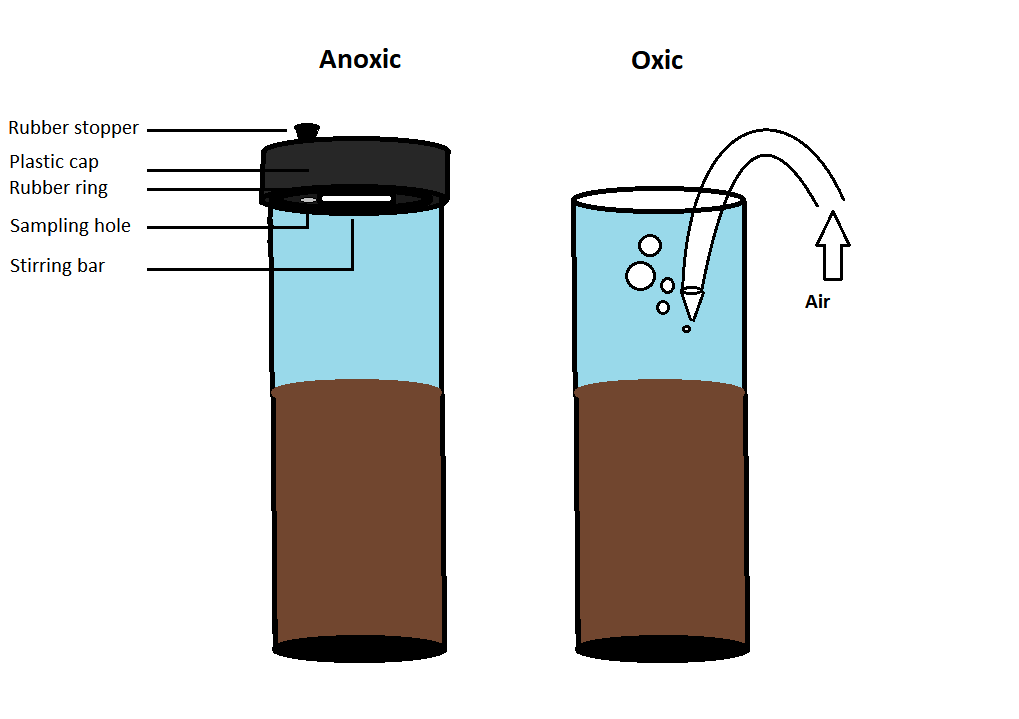
\includegraphics[width=0.4\linewidth]{C:/Users/harmv/Documents/studie/scriptie/Master/Master_Thesis/index/figures/Schematic} 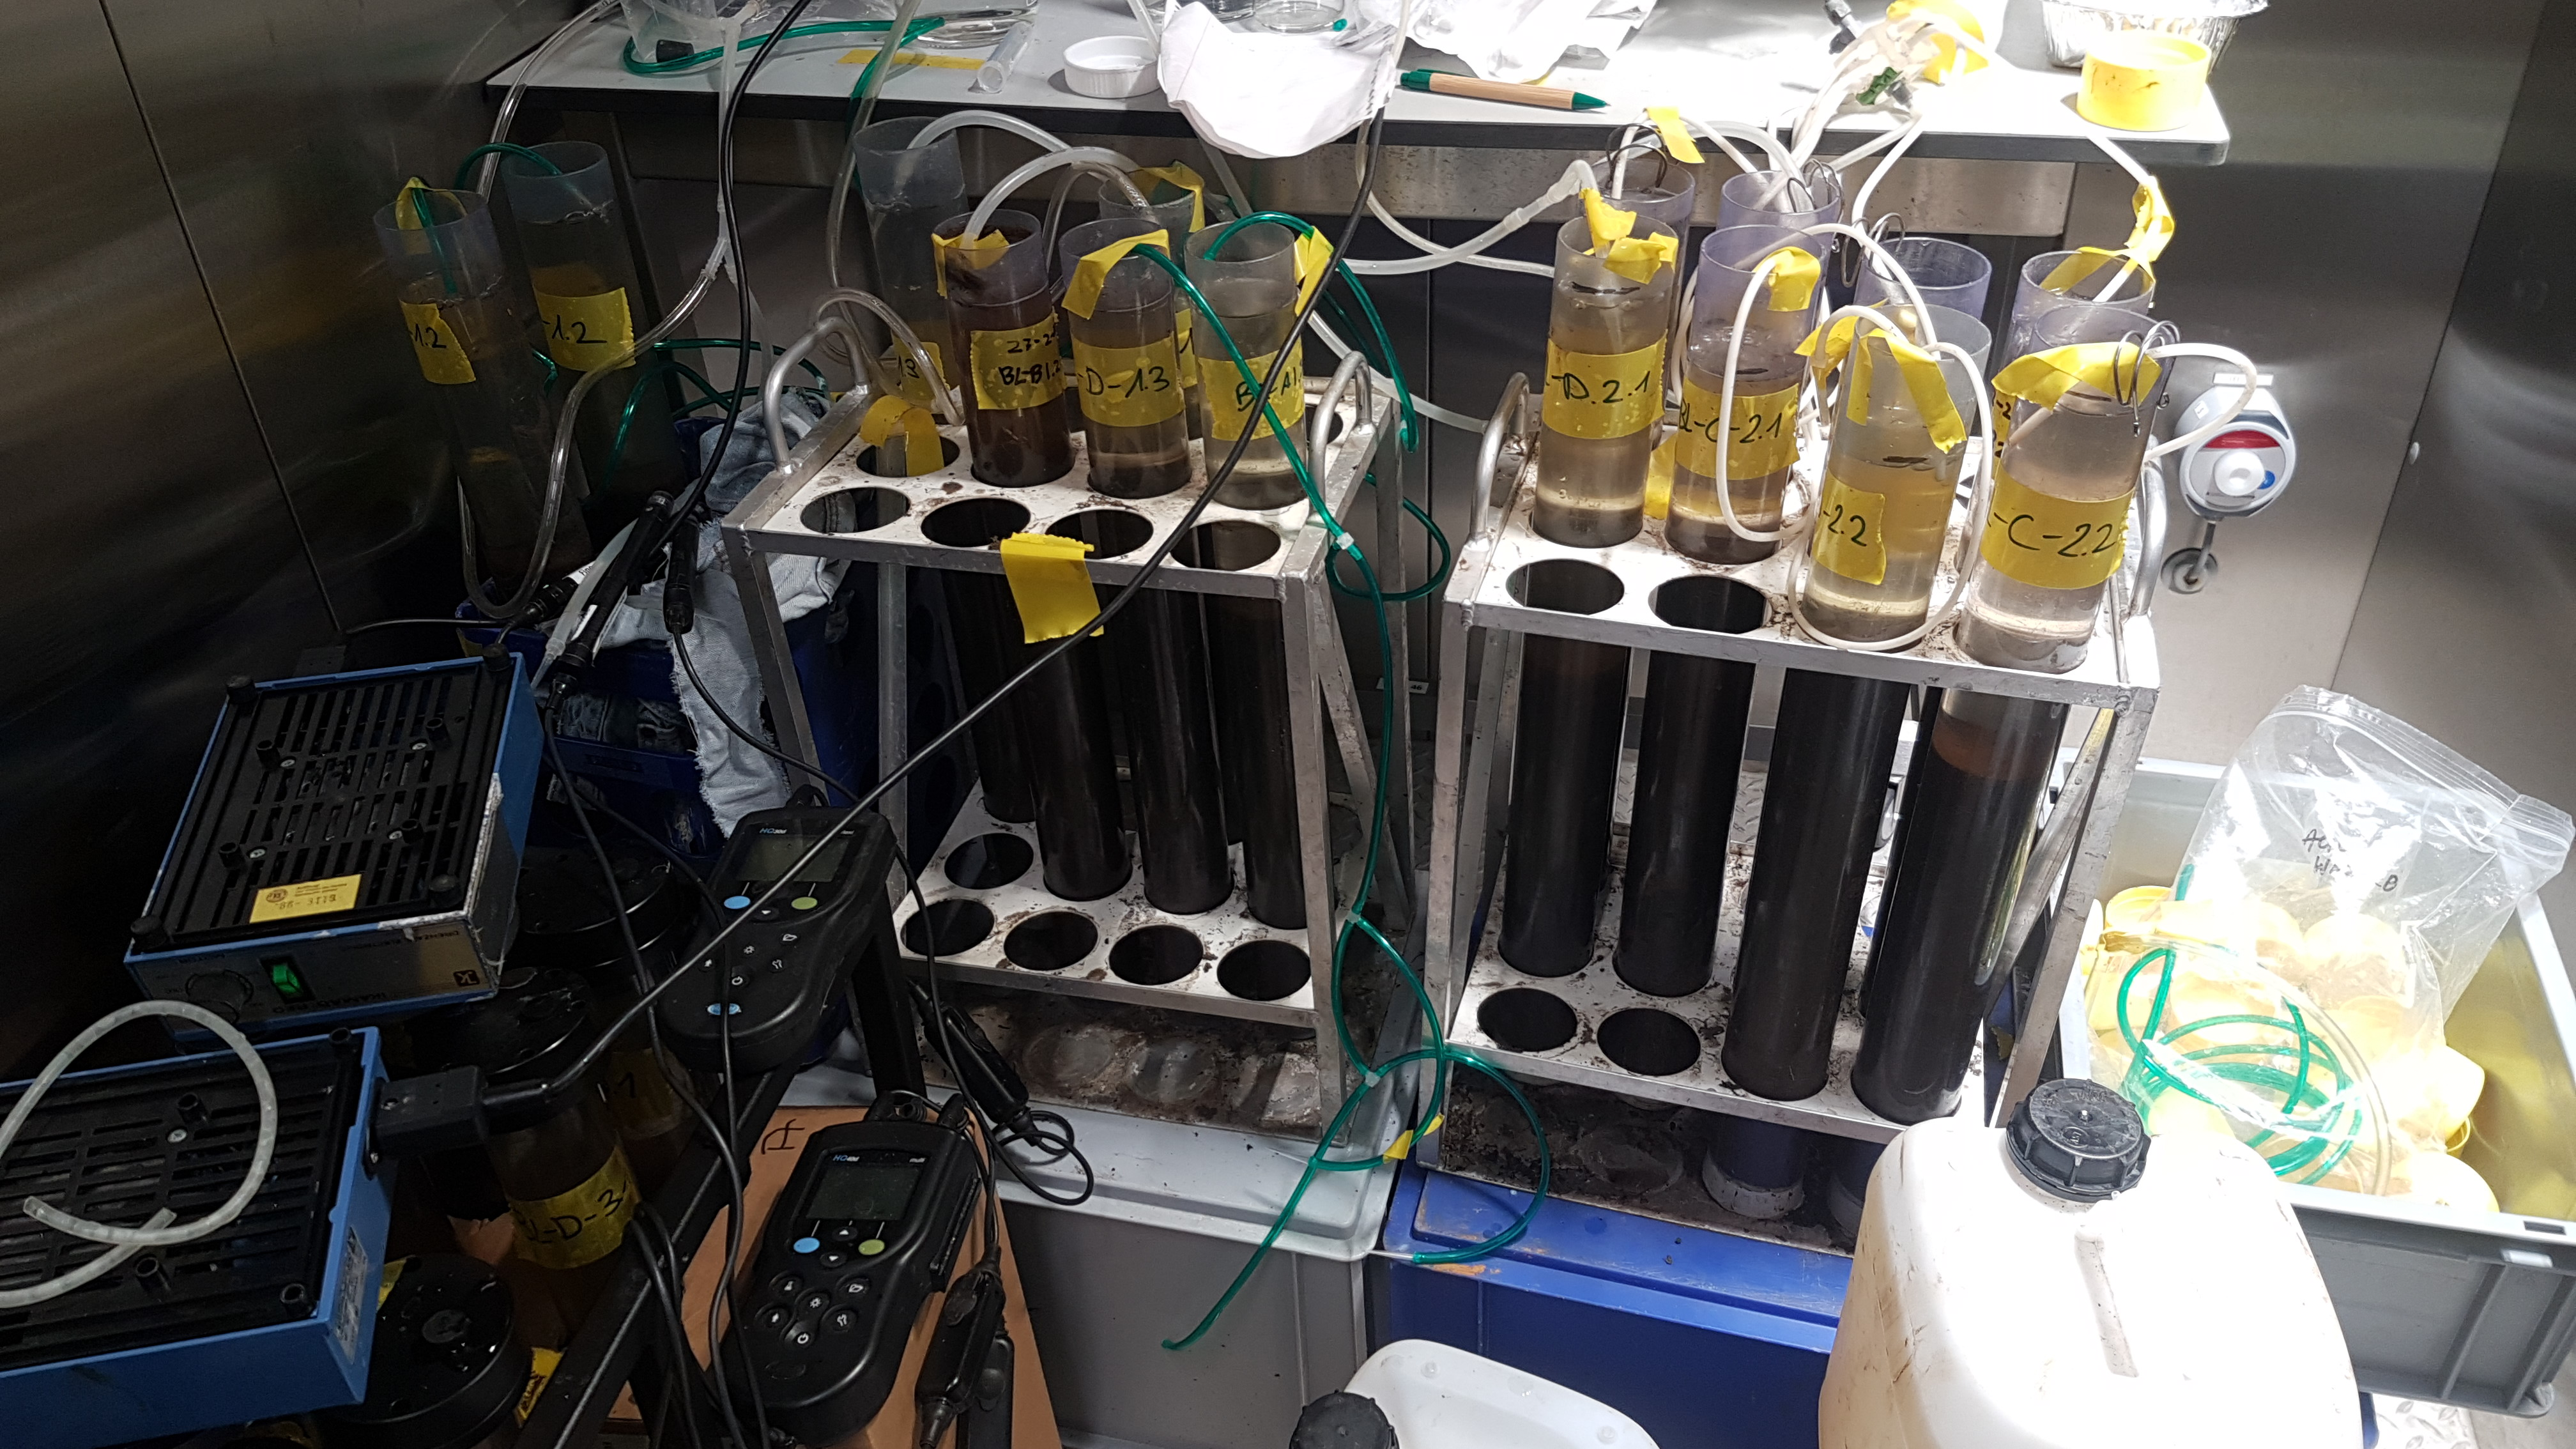
\includegraphics[width=0.4\linewidth]{C:/Users/harmv/Documents/studie/scriptie/Master/Master_Thesis/index/figures/setup} 

}

\caption{Incubating cores to monitor benthic fluxes. Left: Schematic representation of the anoxic and oxic incubations. Right: Photograph of the climate chamber during the experiment. In the center the oxic cores are aerated through tubes, while in the down-left corner the anoxic cores are contnuously stirred by upside-down magnetic stirrers.}\label{fig:setup}
\end{figure}
\hypertarget{analytical-procedures}{%
\subsection{Analytical procedures}\label{analytical-procedures}}

Surface water, incubation samples and porewater were analyzed on phosphate, total iron, ferrous iron (Fe\(^{2+}\)), sulfide and ammonium with spectrophotometry following standardized methods using coloring reagents.(\protect\hyperlink{ref-murphyModifiedSingleSolution1962}{Murphy and Riley 1962}) For P and Fe measurements, as precaution against oxidation, subsamples were acidified after sampling with 1\% 3.75M HNO\(_3\). (\protect\hyperlink{ref-brayPhosphateInterstitialWaters1973}{Bray, Bricker, and Troup 1973}) Calibration lines for ammonium, total iron and Fe\(^{2+}\) were freshly made every day of measurement, while the phosphate calibration line was made once and remeasured. Water samples were also measured by ion chromatography (IC), to quantify common anions including sulfate and nitrate. The diluted extraction solutions gathered during the sequential extraction procedure were analyzed by inductively coupled plasma optical emission spectrometry (ICP-OES). In addition, spectrophotometry was deployed to identify the oxidation state of dissolved iron, which was only possible in the HCl extracted pool, as CBD and concentrated HNO\(_3\) strongly influence the redox potential, and the MgCl and pyrophosphate extracts were exposed to oxygen during the extraction procedure. However, the sediment was kept under nitrogen flow, and the low pH of HCl stabilizes the redox state. Since HCl extracts various different reactive iron species, an evaluation on the redox state is useful. However, many values of Fe\(^{2+}\) were found higher than total iron concentration. Total iron measured with spectrophotometry correlated strongly with ICP-OES Fe data, and is thus considered to be more reliable than the Fe\(^{2+}\) results, which are excluded from this study.

The saturation index (SI), which signifies if a mineral is under- or supersaturated with respect to a certain mineral, and is derived from the equilibrium constant and the activities of the dissolved species of the formation reaction, was calculated for vivianite using the program Mineql 5.0 (\protect\hyperlink{ref-MINEQLChemicalEquilibrum}{{``{MINEQL}+ {Chemical Equilibrum Modeling System},''} n.d.}) with the corresponding data base. As the pH of the pore water has not been measured, the pH was systematically varied between 6.0 and 8.0. For the calculation the average total concentrations of dissolved Fe and P in the pore water of the top 10 cm was used with values of 4 and 200 \(\mu\)M, respectively. The ionic strength was assumed to be 1.0 mM. All other data was processed with R in Rstudio. Concentrations were all converted into \(\mu\)mol per g for solids, and \(\mu\)mol per L for solutions. The incubation data was also converted to mole per unit area by multiplying the measured concentrations by the water volume and dividing by the sediment surface area in the core. From linear regression slopes of these values over time the benthic fluxes were calculated, which were tested on significance with a simple T test with a significance level of 0.05.

\hypertarget{results}{%
\section{Results}\label{results}}

\hypertarget{surface-water}{%
\subsection{Surface water}\label{surface-water}}

The surface water measured \textit{in situ} at both the treated and non treated locations had dissolved oxygen concentrations of 9.5-10.5 mg/L and pH levels of around 8. While no significant difference between treated and non-treated locations, water conditions did vary between the locations closer (C and D) and further away (A and B) from the water inlet, due to a significantly higher electric conductivity at locations A and B (\(438\pm9\mu\)S and \(451\pm5\mu\)S), than measured at locations C and D (\(395\pm15\mu\)S and \(397\pm5\mu\)S).
\begin{figure}

{\centering 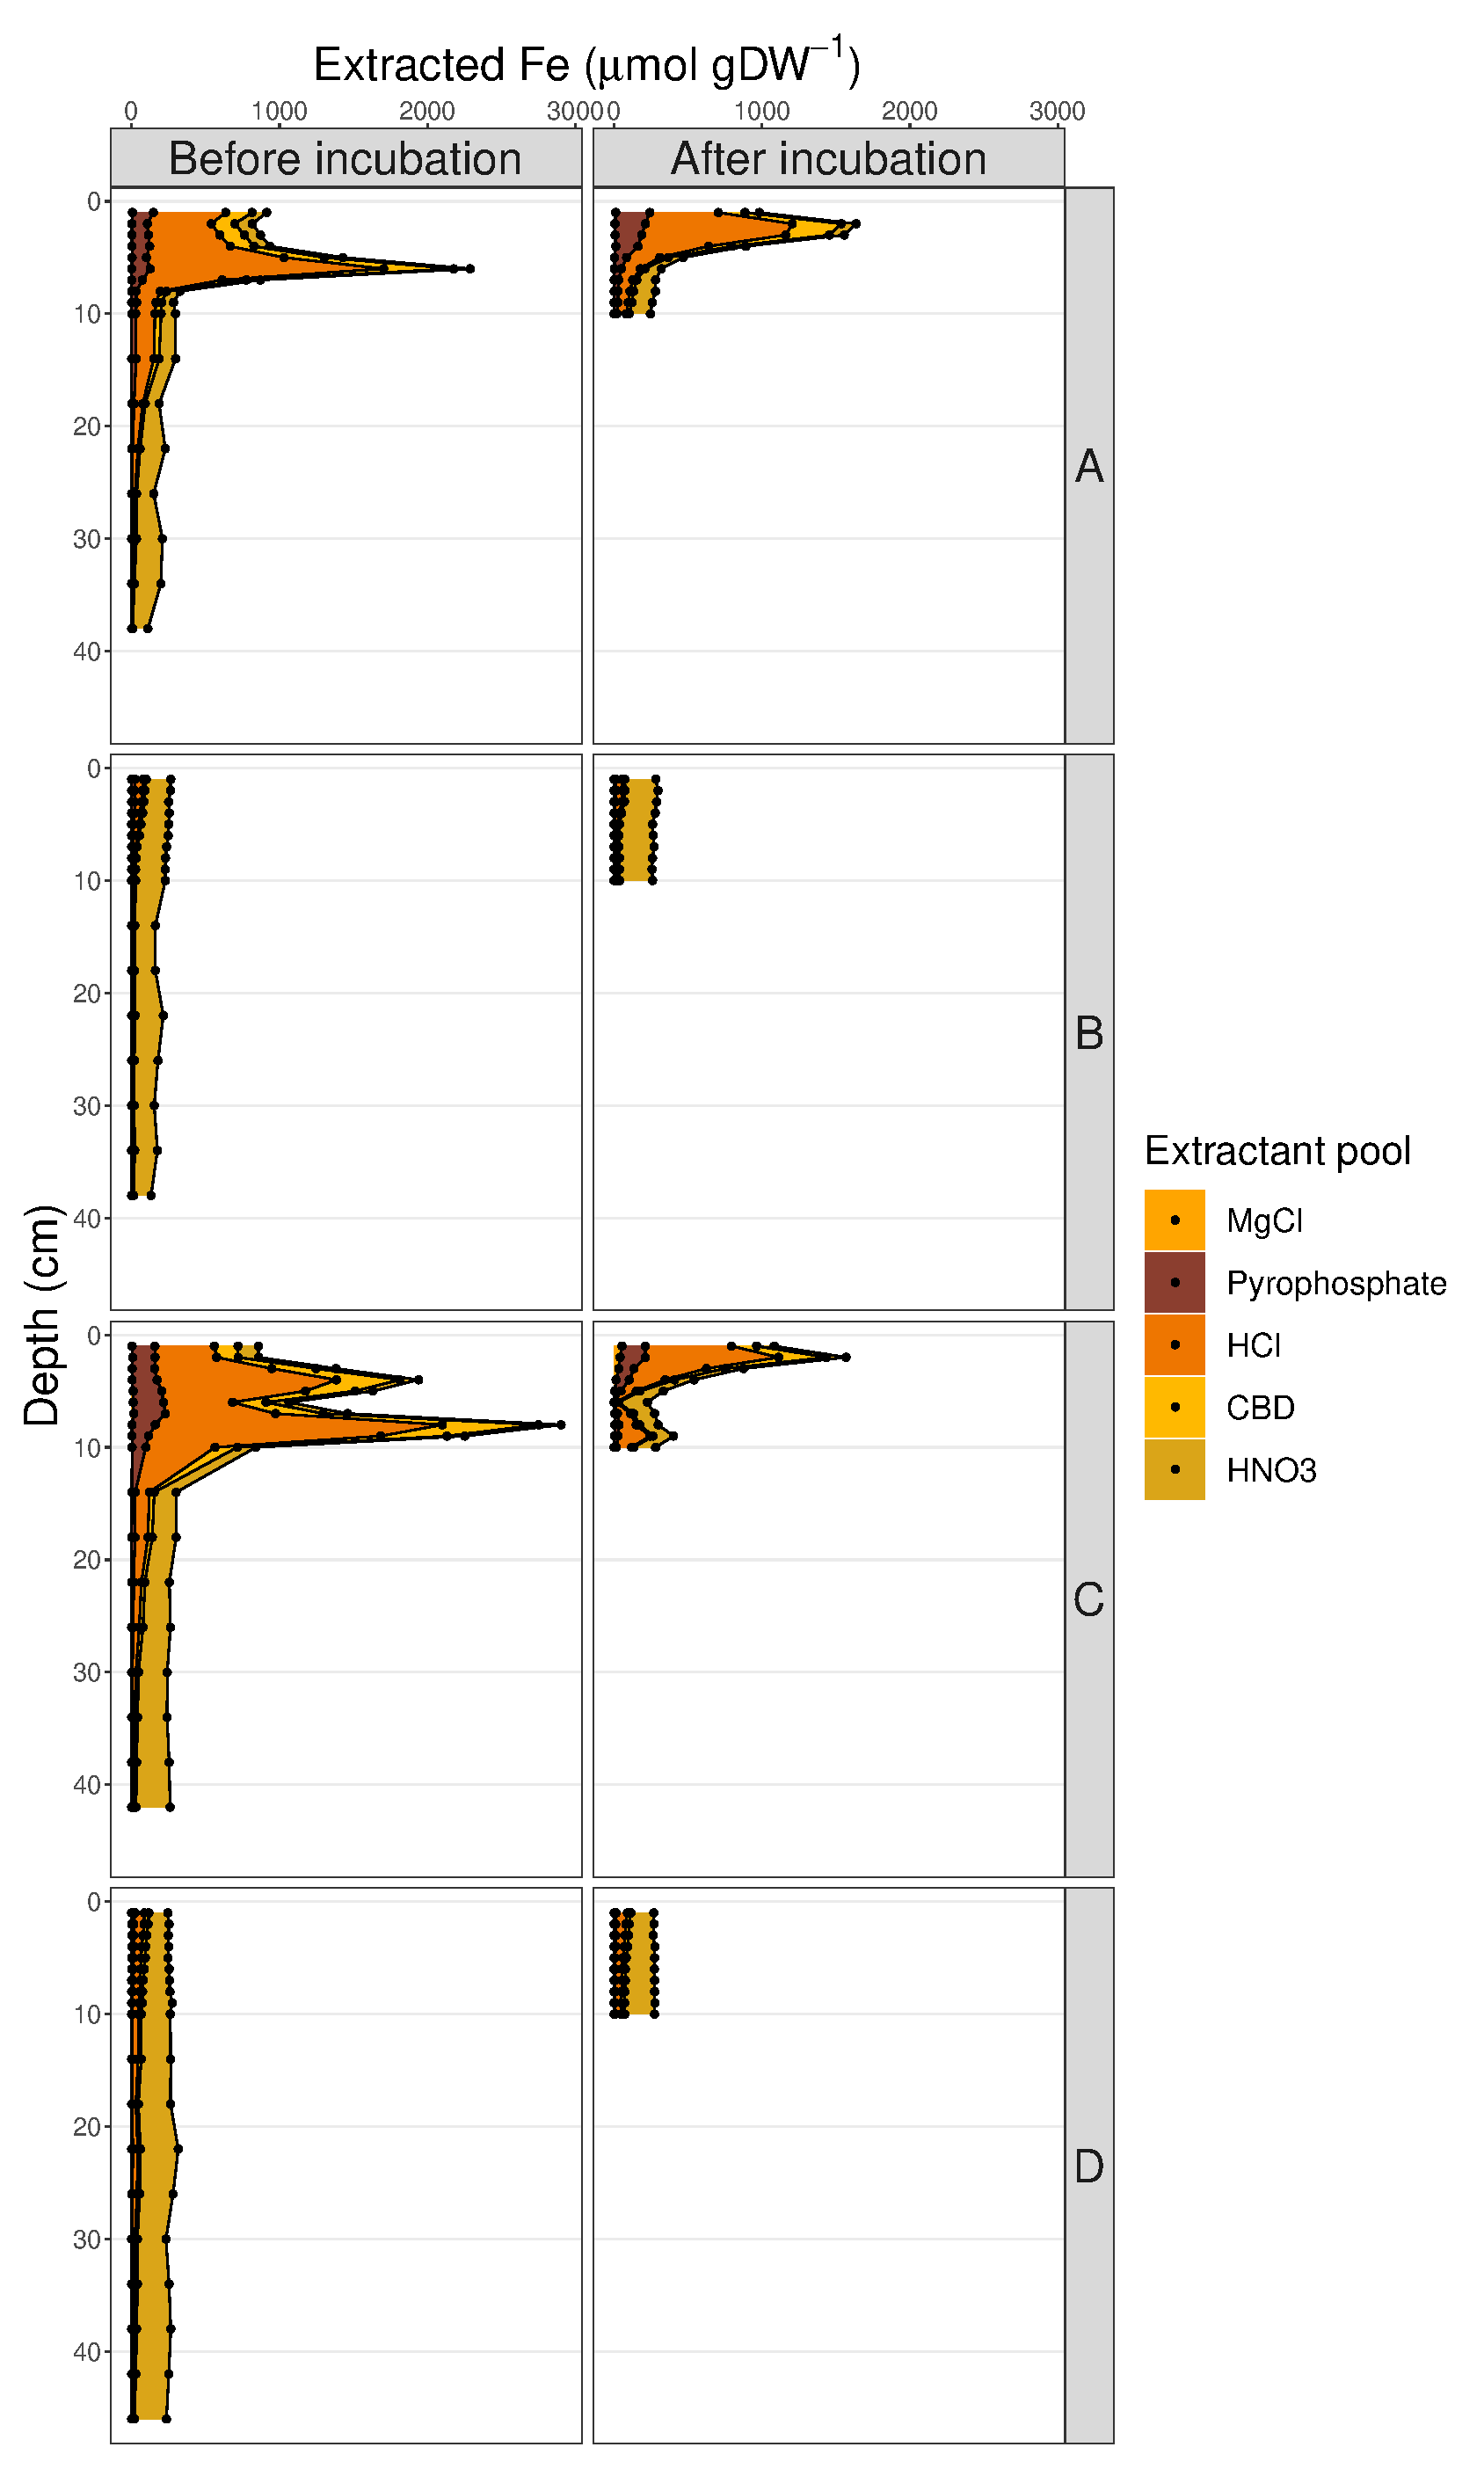
\includegraphics[width=0.45\linewidth]{C:/Users/harmv/Documents/studie/scriptie/Master/Master_Thesis/index/figures/seq_extr_Fe_2} 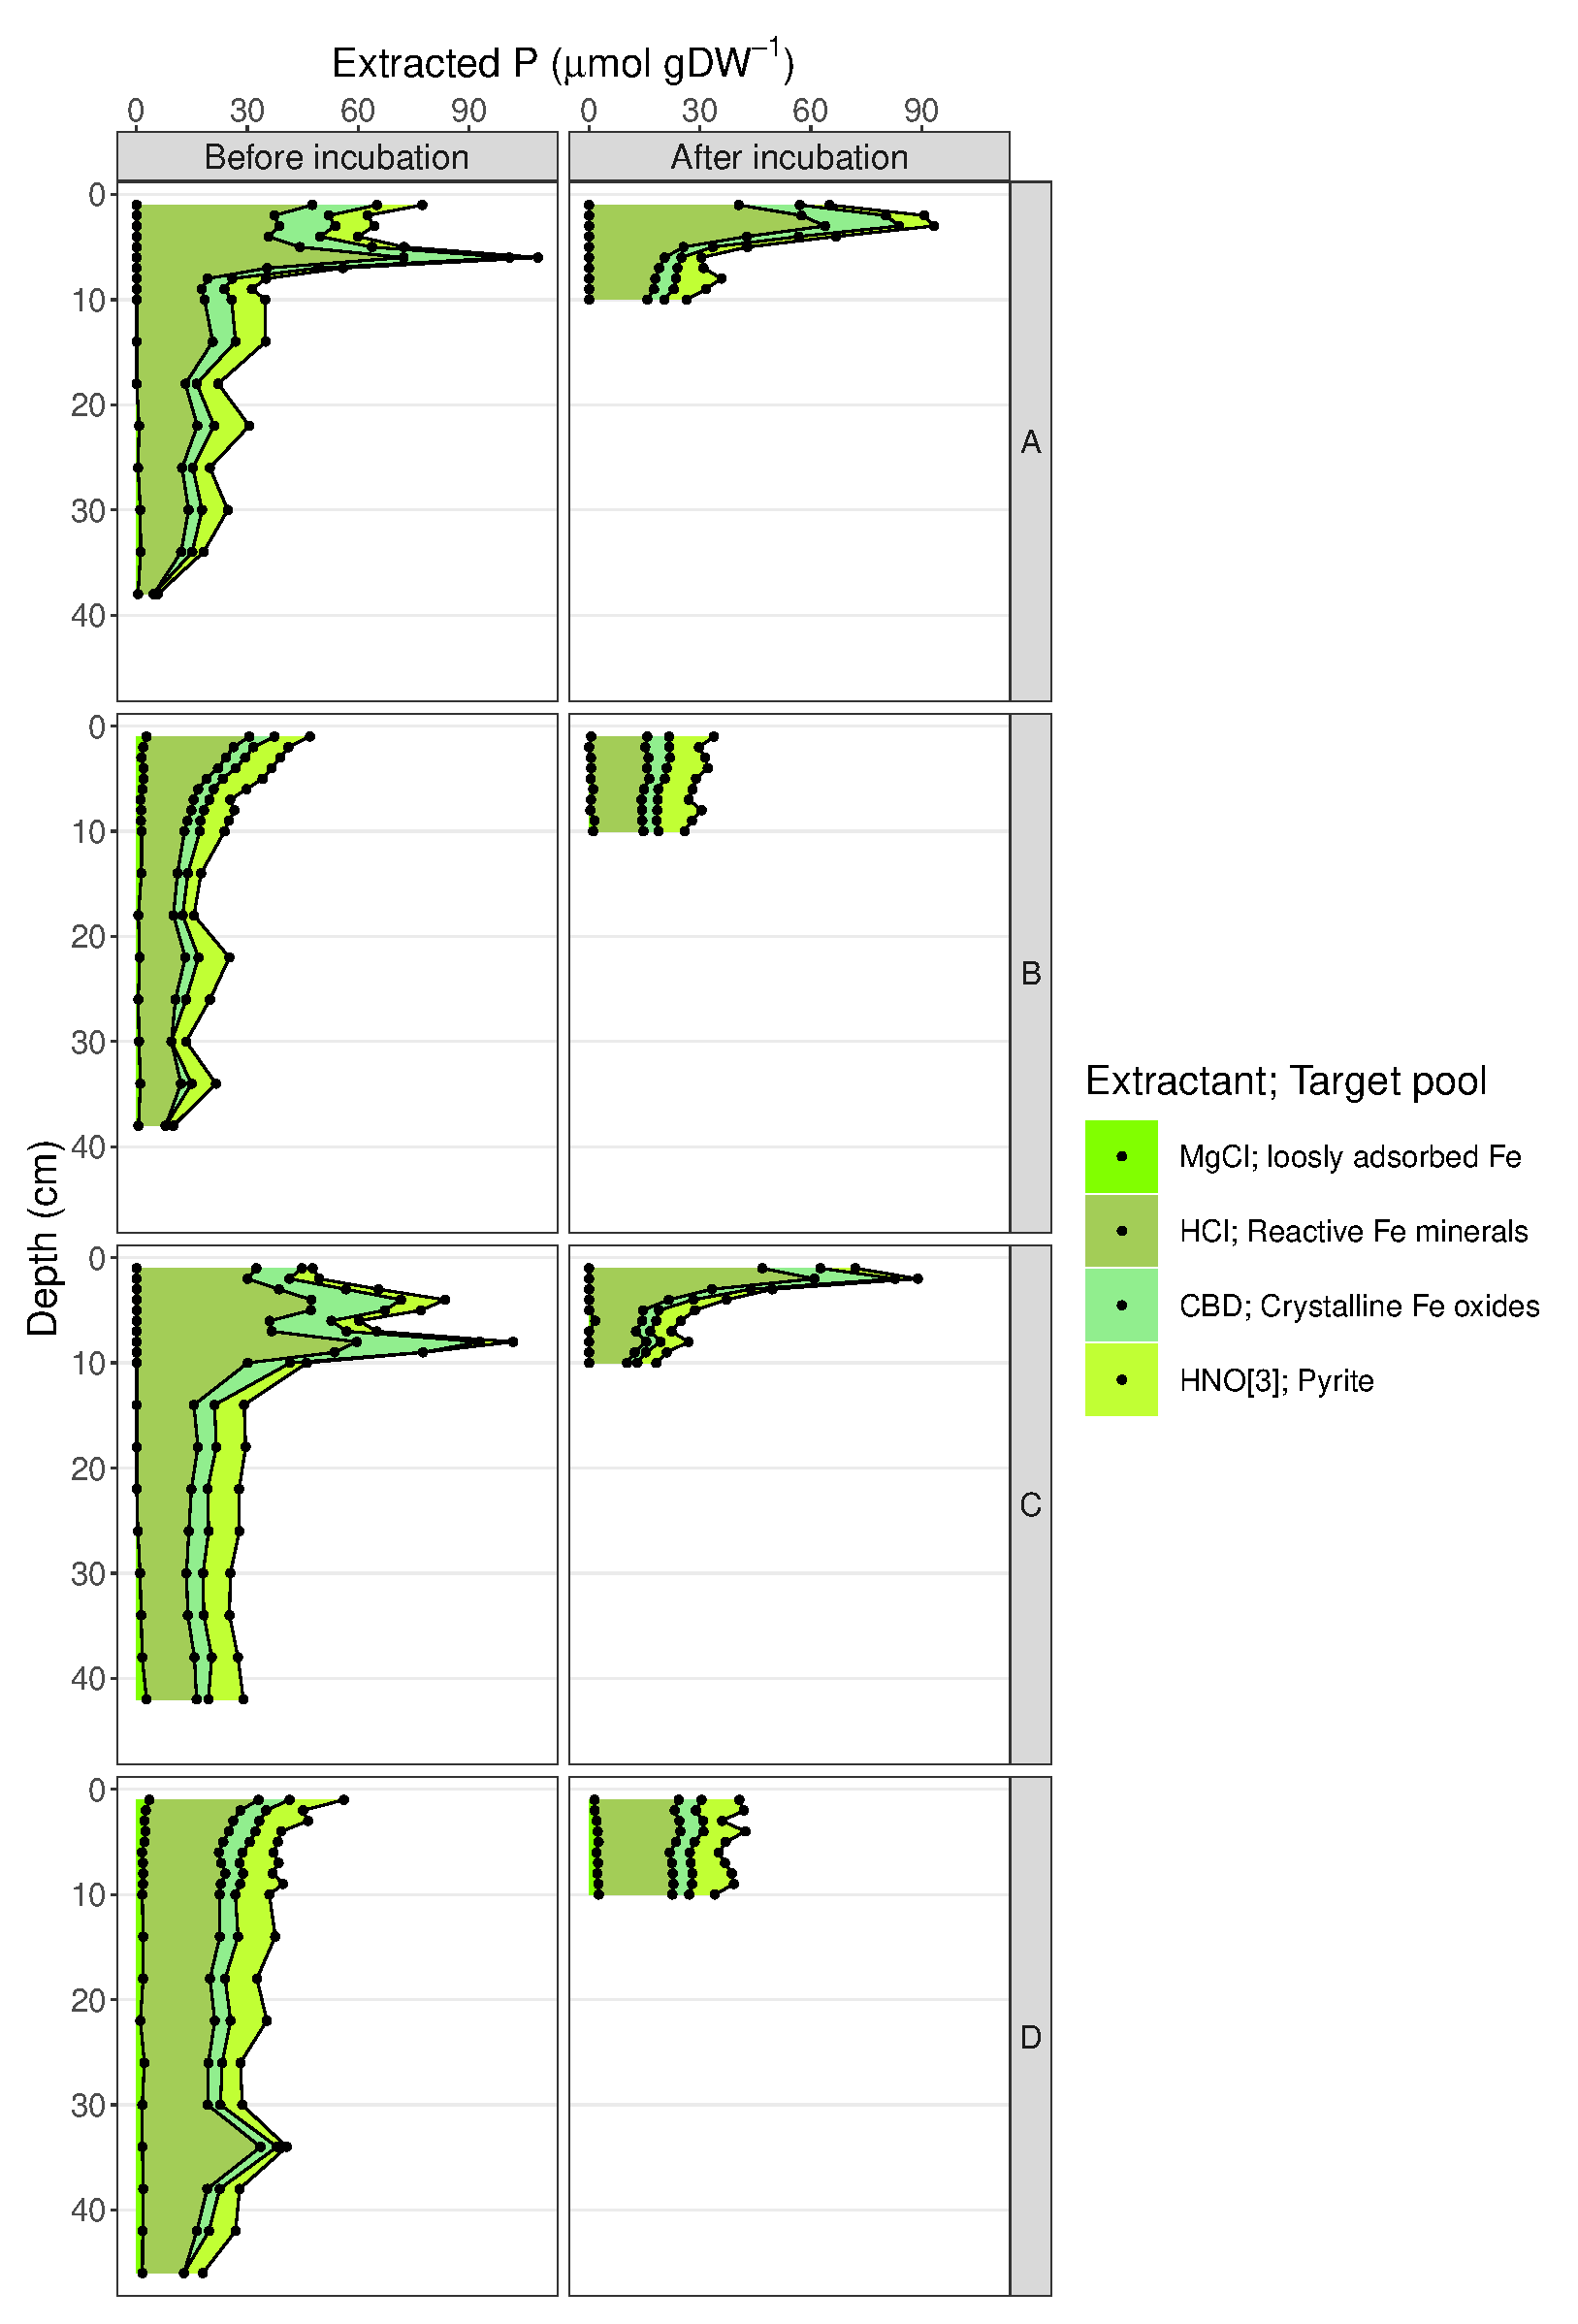
\includegraphics[width=0.45\linewidth]{C:/Users/harmv/Documents/studie/scriptie/Master/Master_Thesis/index/figures/seq_extr_Fe_3} 

}

\caption{Sequential extraction results. The extracted Fe and P for each extraction step is plotted as function of depth. Left panel shows the extracted Fe in each pool, the right panel the P.  The stacked and coloured integrals represent the relative size of the corresponding extacted pool and the total width the sum of all pools. The pyrophosphate extraction was performed in parallel, and is substracted from the HCl pool in the Fe data.   }\label{fig:seq}
\end{figure}
\hypertarget{sediment-analysis}{%
\subsection{Sediment analysis}\label{sediment-analysis}}

Addition of Fe-containing by-products resulted in significantly higher Fe content of the sediments. The untreated sediment contains about 2wt\% of Fe uniformly distributed over depth, whereas the Fe content in the treated sediment varies considerably with depth and reaches up to 25wt\% at certain intervals, but is mainly found in the shallow (\textless10cm) sediment. In total, the first 10cm of sediment of the treated cores contain 1550mg and 3580mg (cores from locations A and C, respectively) of Fe, significantly higher than the Fe content of the non-treated cores which in the top 10cm adds up to 490mg and 590mg (cores from locations B and D, respectively).

In figure \ref{fig:seq}, left panel, which shows Fe concentrations acquired by sequential extraction, is shown that the largest Fe pool extracted in the treated sediment is the HCl extractable pool (average 50-60\% of total Fe in top 10cm), in contrast to untreated sediment, where the HCl extracted Fe is only about 10\% of the total Fe in the 10 cm, and most Fe is extracted by HNO\(_3\) (40-60\%). The HNO\(_3\) extracted Fe content is constant with depth in all cores (116-223 \(\mu\)mol g\(^{-1}\), \(\sigma=\) 25 \(\mu\)mol g\(^{-1}\)), and independent of variations in total Fe. In contrast, values of extracted Fe in all fractions except HNO\(_3\) peak within the first 10cm of sediment, then decrease with depth. This amounts to average amounts of Fe extracted in the non-treated cores by HCl, pyrophosphate and CBD extractions 2-10 times higher in the top 10cm (HCl: 54 \(\pm\) 22 \(\mu\)mol g\(^{-1}\); pyrophosphate: 12 \(\pm\) 7 \(\mu\)mol g\(^{-1}\); CBD: 20 \(\pm\) 6 \(\mu\)mol g\(^{-1}\)) than in deeper sediment (HCl: 18 \(\pm\) 11 \(\mu\)mol g\(^{-1}\); pyrophosphate: 2.5 \(\pm\) 2.1 \(\mu\)mol g\(^{-1}\); CBD: 13 \(\pm\) 4 \(\mu\)mol g\(^{-1}\)), and in the treated cores approximately 20 times more (\emph{shallow} HCl: 840 \(\pm\) 520 \(\mu\)mol g\(^{-1}\); pyrophosphate: 123 \(\pm\) 55 \(\mu\)mol g\(^{-1}\); CBD: 240 \(\pm\) 160 \(\mu\) mol g\(^{-1}\); \emph{deep} HCl: 36 \(\pm\) 30 \(\mu\)mol g\(^{-1}\); pyrophosphate: 6 \(\pm\) 7 \(\mu\)mol g\(^{-1}\); CBD: 17 \(\pm\) 7 \(\mu\)mol g\(^{-1}\)). The size of all Fe pools other than HNO\(_3\) is proportional to the total Fe content with a relatively stable distribution between the pools: For the non-treated shallow 10cm of sediment the average molar ratio between the HCl, pyrophosphate and CBD pools is respectively 6:1:2, though deeper in the sediment this ratio changes gradually in favor of the CBD pool (MgCl\(_2\) pools are negligible, and often below the detection limit). The treated sediment has an average HCl-pyrophosphate-CBD ratio of 7:1:2 in the top 10cm, which means the treated cores contain relatively more HCl extractable Fe compared to the untreated sediment.

In addition to sediment from cores which were sliced and processed directly after the field campaign, selected cores used in the benthic flux experiment were partly sliced and analyzed by sequential extraction after the experiment ended, of which the results are shown in the right columns in figure \ref{fig:seq}. HNO\(_3\) extracted Fe content in non-treated cores are roughly 20\% higher after anoxic incubation than in the fresh cores, while the HCl and pyrophosphate pools are 5-50\% smaller.

Phosphate extracted during the sequential extractions correlates with the total Fe content, and with the HCl pool. Most P (30-50\% of total P) is extracted by HCl in all cores. In the treated cores this is the largest pool of Fe as well, but HCl extracted Fe is just a small fraction in the non-treated cores, still the extracted P is largest in this pool. (Fig. \ref{fig:seq}, right panel) The treated sediment contain more P extracted with HCl than the untreated sediment (on average 20-100\% more at shallow depth; respectively 54-75mg and 33-48mg total P), particularly at depths where the Fe content is highest, but the contrast is not as large as for the Fe content, which can be an order of magnitude larger.
\begin{figure}

{\centering \includegraphics[width=1\linewidth]{C:/Users/harmv/Documents/studie/scriptie/Master/Master_Thesis/index/figures/profiles} 

}

\caption{Porewater concentrations as function of depth. The plots share the y axis which represents the sediment depth, while the x axes are scaled individually for each dissolved species. Cores from treated locations are shown in red, non-treated reference locations in blue. Top row shows cores sliced directly after sampling, the bottom row after two months incubating under anoxic conditions. Iron, phosphate, slufide and ammonia were measured with photospectometry, sulfate and nitrate with IC.}\label{fig:pwprofiles}
\end{figure}
\hypertarget{porewater-analysis}{%
\subsection{Porewater analysis}\label{porewater-analysis}}

Similar to the solid phase composition, addition of Fe containing by-products was also reflected in the composition of the sediment pore waters. Porewater of the non-treated cores contain very little Fe (\textless{} 10 \(\mu\)M), but porewater Fe concentrations in the treated cores were high (\textgreater30 \(\mu\)M up to 350 \(\mu\)M, see fig.~\ref{fig:pwprofiles}) at depths with high solid iron content, and found in both the 2+ and 3+ oxidation state. The ratio Fe\(^{3+}\)/Fe\(^{2+}\) in the top 10 cm is relatively high and exceeds 1 at certain depths. Concurrent with the solid Fe content, dissolved iron is highest at 1 - 10 cm depth, and subsequently decreases with depth. Below this sediment layer where solid iron is concentrated, dissolved Fe in the porewater is predominantly found as Fe\(^{2+}\).

Phosphate concentrations in the porewater exhibit a trend opposite to that of Fe: P concentrations in porewater of non-treated cores are much higher (20-240 \(\mu\)M) than in the treated cores, where P concentrations are low (\textless{} 5 \(\mu\)M). Similar to the P concentration decrease as result of added Fe, sulfide concentrations are considerably lower in treated cores (\textless{} 1 \(\mu\)M), opposed to high sulfide concentrations in the porewater of untreated sediment (5-100 \(\mu\)M). This effect persists deep in the core, below the shallow zone where sediment is enriched with Fe.
In addition, the decrease in sulfate concentration with depth in the porewater was steeper in locations C and D compared to A and B.( Fig. \ref{fig:pwprofiles})
\begin{figure}

{\centering 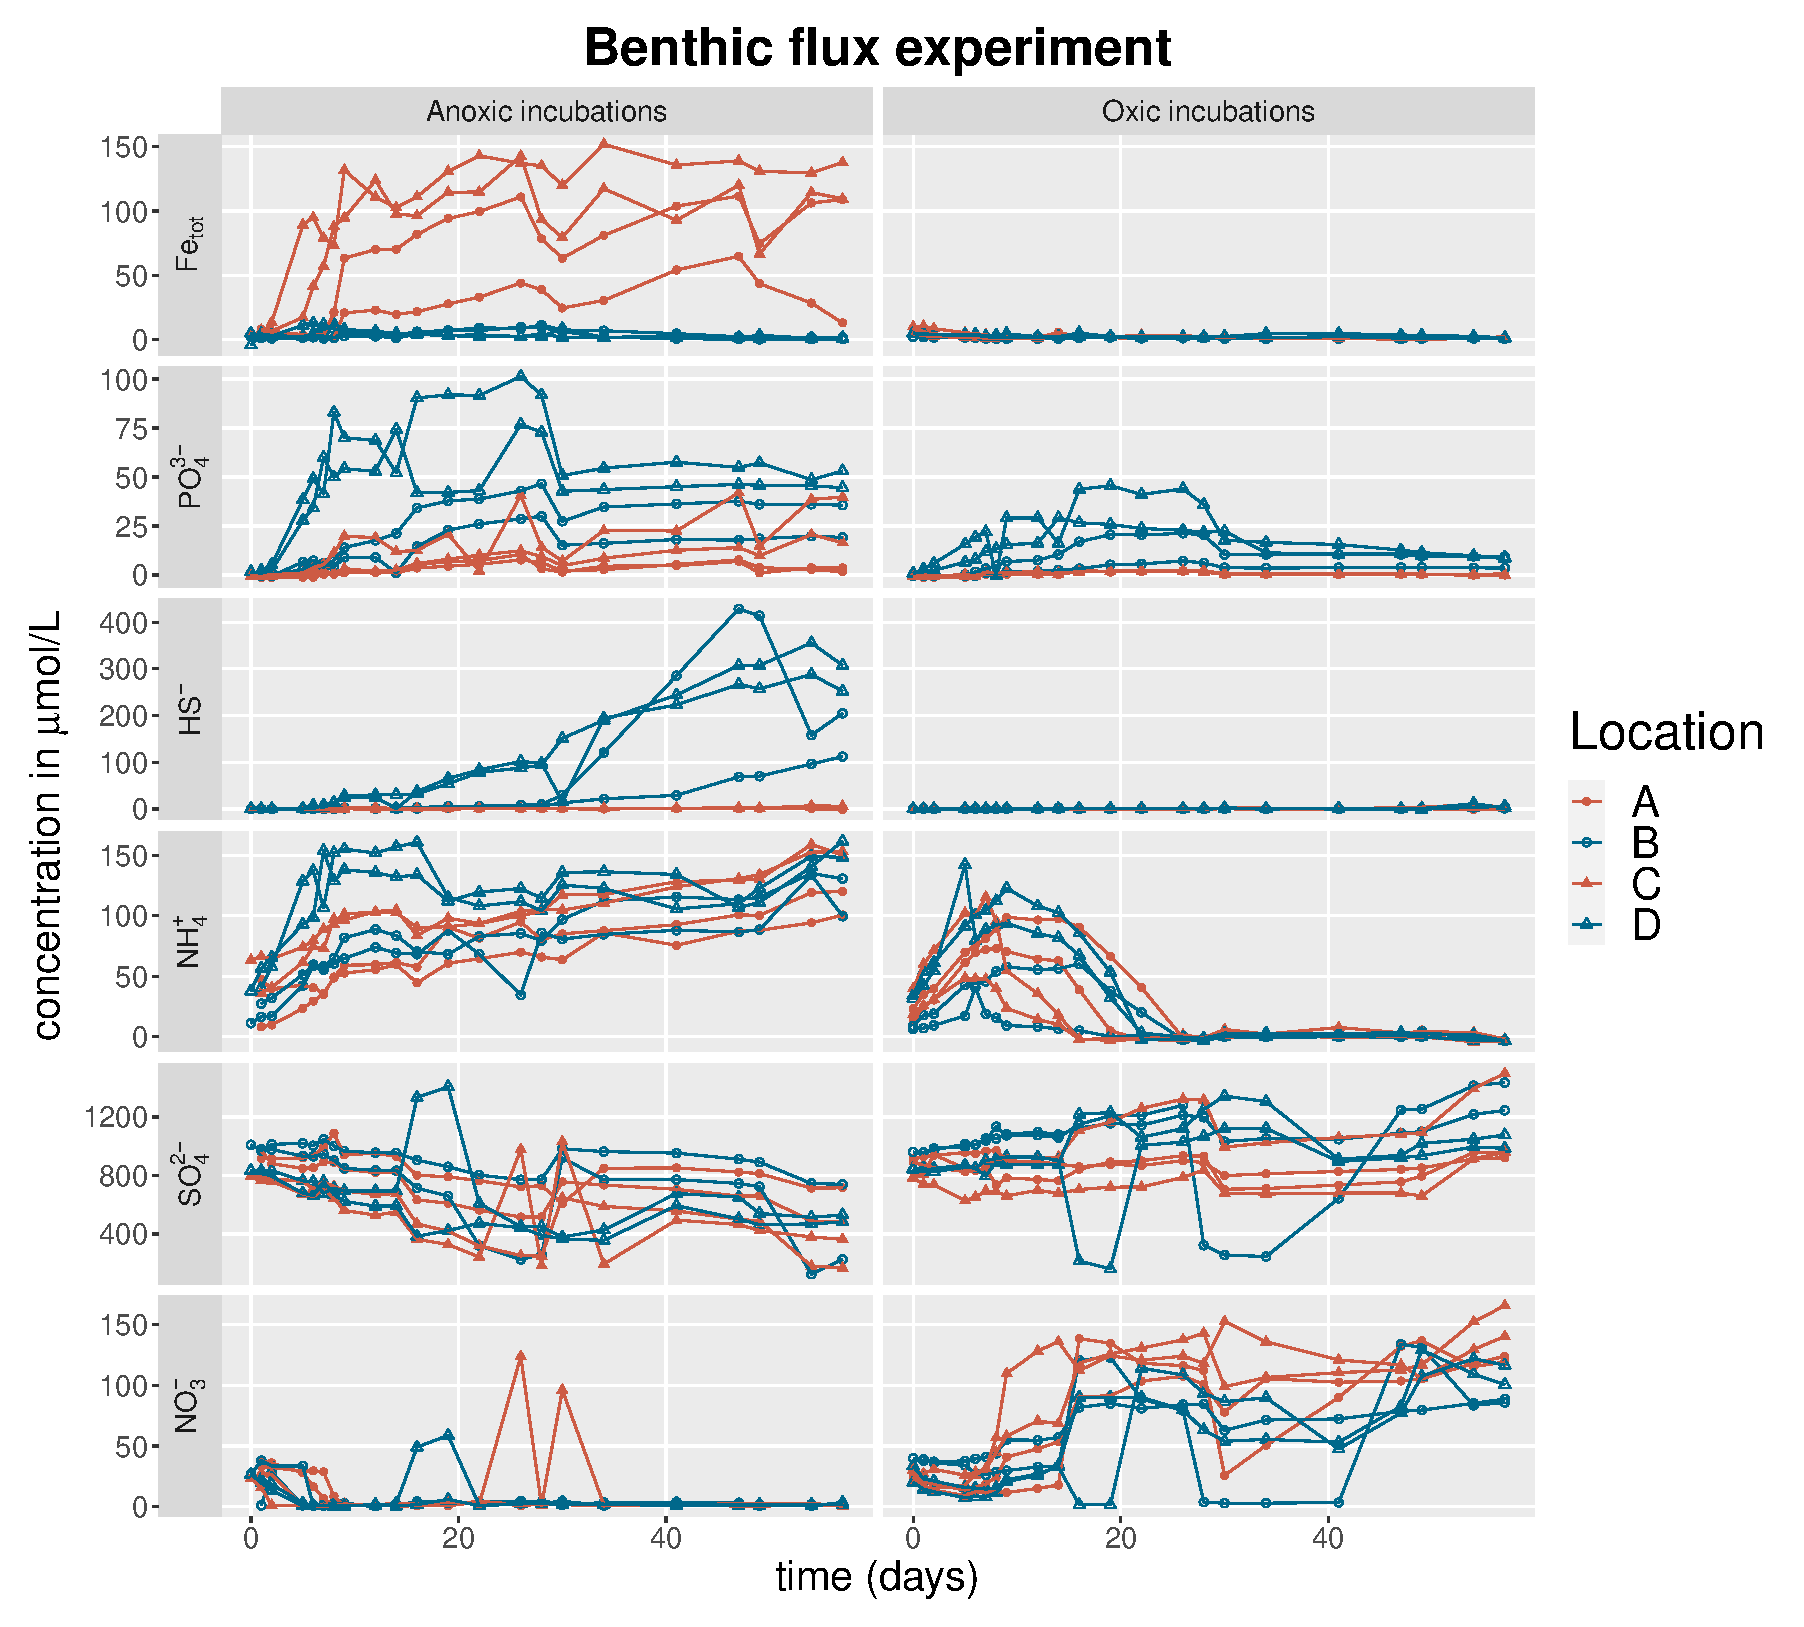
\includegraphics[width=0.85\linewidth]{C:/Users/harmv/Documents/studie/scriptie/Master/Master_Thesis/index/figures/IC_incubations_1} 

}

\caption{Time evolution of the concentrations of solutes in overlying water of incubated cores. Cores with anoxic conditions induced during the experiment (left colum) are compared with cores kept oxic by continue aeration (right column). The main goal was to study the difference in benthic fluxes from treated sediment, here in red, in relation to untreated sediment, displayed in blue. There are two treated and two untreated locations,  every location is incubated in duplo. The scale of the y axis is different for each parameter, while the x axis representing time in days is the same for all.}\label{fig:incubations}
\end{figure}
\hypertarget{benthic-flux-measurements}{%
\subsection{Benthic flux measurements}\label{benthic-flux-measurements}}

The benthic flux experiment shows that Fe treatment changes the release of P and Fe significantly over time, as P release is suppressed while Fe increase is enhanced. The increase of P over time was highest in non-treated cores, and remain much lower in surface water of treated cores. Furthermore, lowering the redox conditions of the overlying water increases P release. Fe release from the treated sediment is dependent on redox conditions as well, and is highest in the anoxic cores. The increase in Fe in the treated cores is characterized by high flux (1-3 mmol m\(^{-2}\) day\(^{-1}\)) at the start of the experiment, followed by a much lower flux after 1-2 weeks (Fig. \ref{fig:incubations}). The non-treated cores on the other hand, exhibit much lower, but still significant Fe fluxes, particularly in the D core, where they reach up to 200 \(\mu\)mol m\(^{-2}\) day\(^{-1}\) (Table \ref{tab:flux}). An initial increase in Fe concentration is in the non-treated cores is followed by a gradual decrease, while at the same time the sulfide concentration increases. The increase in sulfide in low redox conditions is coupled with a decrease in sulfate concentration. Sulfide concentrations are not increasing in th treated cores, though sulfate concentration decreases at the same rate as in the non-treated cores under anoxic conditions (0.6-1.6 mmol m\(^{-2}\) day\(^{-1}\)). Finally, nitrogen, in the form of ammonium (NH\(_4^+\)) and nitrate (NO\(_3^-\)), is less influenced by the treatment. After an initial high ammonium flux (1-3 mmol m\(^{-2}\) day\(^{-1}\)), the increase slows down, and with oxygen available, nitrification dominates in the oxic cores. While this pattern is found in all cores, the ammonium production rate appears to be smaller during the initial rise, but larger during the long-term increase in the treated cores.
\begin{table}[ht]
\centering
\begin{tabular}{rl|rrrrrrr||rrr|}
  \toprule
  & &\multicolumn{10}{l}{\textbf{Benthic fluxes in mmol m$^{-2}$ day$^{-1}$}} \\
  \hline
  & & \multicolumn{7}{c}{Anoxic incubations} & \multicolumn{3}{c}{Oxic incubations} \\
 &  &  \multicolumn{2}{c}{Fe$_{tot}$} & PO$_4^{3-}$ & \multicolumn{2}{c}{NH$_{4}^+$} & HS$^-$ & SO$_4^{2-}$ & 
 PO$_4^{3-}$ & NH$_{4}^+$ &  NO$_3^-$ \\ 
 & \footnotesize{Time interval:} & \textbf{I} & \textbf{III} & \textbf{II} & \textbf{I} & \textbf{III} & \textbf{III} & \textbf{III} & \textbf{II} & \textbf{I} &  \textbf{III} \\
  \hline
& A & 1.09$\ast$ & 0.22 & 0.11 & 1.48 & 0.30 & 0.00 & -1.20 & 0.02 & 1.34 &  0.29 \\ 
&  & 0.12$\ast$  & 0.12$\ast$ & 0.08 & 0.15$\ast$ & 0.27 & -0.00$\ast$ & -1.11 & 0.02 & 0.81 &  0.18 \\ \hline
& B & 0.08$\ast$ & -0.01$\ast$ & 0.23 & 1.33 & 0.18 & 0.42 & -0.55$\ast$ & 0.07 & 0.23$\ast$ &  0.11 \\ 
&  & 0.01$\ast$ & -0.01$\ast$ & 0.33 & 0.96 & 0.19 & 1.15 & -1.23$\ast$ & 0.24 & 1.08 & 0.17$\ast$ \\ \hline
& C & 2.90 & 0.14 & 0.10 & 0.94 & 0.25 & 0.02 & -1.42 & 0.01 & 0.27$\ast$ &  0.03$\ast$ \\ 
&  & 2.88 & -0.00$\ast$ & 0.15$\ast$ & 2.00 & 0.29 & 0.02 & -0.71$\ast$ & 0.03 & 0.18$\ast$ &  0.29 \\ \hline
& D & 0.20$\ast$ & -0.03 & 0.39$\ast$ & 2.45 & 0.02$\ast$ & 1.32 & -1.58$\ast$ & 0.31 & 1.40$\ast$  & 0.46 \\ 
&  & 0.15$\ast$ & -0.03 & 0.95 & 3.31 & -0.09$\ast$ & 1.72 & -0.47$\ast$ & 0.22 & 0.96  & 0.16 \\ 
   \hline
   & & \multicolumn{10}{l}{\scriptsize{$\ast$ T test P value of linear model slope above 0.05}} \\
   \multicolumn{12}{l}{\footnotesize{\textbf{I}: First 10 days}} \\
   \multicolumn{12}{l}{\footnotesize{\textbf{II}: First 25 days}} \\
   \multicolumn{12}{l}{\footnotesize{\textbf{III}: After a week}} \\
   \bottomrule
\end{tabular}
\caption{Estimations of benthic fluxes for selected species during incubation on various timescales. The fluxes are computed by deriving the slope of a linear regression over time within certain time intervals, which can be found in the table by roman numbers. The different time intervals were chosen based on periods with relatively constant increase observed in the incubation data. Important to note is that the calculated fluxes have a high degree of uncertainty, the values with an asterix are statistically not significantly different from 0.}
    \label{tab:flux}
\end{table}
\hypertarget{discussion}{%
\section{Discussion}\label{discussion}}

\hypertarget{effect-fe-treatment-of-biogeochemical-processes-in-the-sediment}{%
\subsection{Effect Fe treatment of biogeochemical processes in the sediment}\label{effect-fe-treatment-of-biogeochemical-processes-in-the-sediment}}

The peat meadow system in this study is generally very poor in Fe, and the Fe content in the original sediment attributes to less than 2\% of the dry weight. The majority of the Fe in the untreated cores was extracted in the HNO\(_3\) pool, most likely as result of crystalline sulfide phases such as pyrite formed in the sediment, where high sulfide concentrations are found in the porewater. Phosphate is scarcely found within sulfide phases, so the presence of phosphate in this pool would be better explained as consequence of oxidation of the organic matrix during the extraction, where concentrated HNO\(_3\) can act as oxidator mineralizing OM and P is mobilized. Fe and phosphate bound electrostatically to organic matter would have been extracted in earlier extraction steps, and do not influence these results. (\protect\hyperlink{ref-donisaCombinationDiferrentExtractants2007}{Donisa, Steinnes, and Mocanu 2007})

Addition of Fe drastically changed the composition of the sediment and porewater. The top 10cm of treated cores show Fe contents up to 20 wt\%, and in contrast to the Fe in the untreated sediment which is immobilized in stable sulfide phases, the added Fe is mostly found in the reactive HCl pool. Concurrent with the HCl pool, significant Fe extracted from the treated sediment was found in the pyrophosphate and CBD pools. Pyrophosphate extracts Fe associated with organic matter (Fe-OM) by solubilising organic substances, so it shows that Fe-OM is present ubiquitously when sufficient Fe is available, and does not correlate with total Fe in sediment or porewater. (\protect\hyperlink{ref-claffSequentialExtractionProcedure2010}{Claff et al. 2010}) In fact, the abundance of Fe in the pyrophosphate pool decreases with depth below 6 cm, above the depth at which the total Fe in sediment peaks. This can be explained if pyrophosphate extractable Fe-OM in deeper sediment is limited by the availability of reactive organic substances rather than the Fe concentration, which contradicts with the fact that organic matter is abundant even in deeper layers. Alternatively, it could be that Fe is still complexed in deeper sediment where Fe is available, but with less reactive forms of organic matter and thus less extractable with pyrophosphate.

Because of meso-scale heterogeneity of horizontal Fe sludge distribution in the treated ditch, the Fe content varies greatly between cores, and absolute size of the pools can therefore not be compared. The variation in Fe content also explains the difference in vertical Fe distribution between cores, as larger clumps of Fe sludge sink deeper in the sediment. Even though the total Fe content in cores from treated locations varies between cores from the same location, the composition of the added Fe-containing by-products at the time of treatment was the same everywhere. In addition, the ratio between the pyrophosphate, HCl, and CBD pools appears to be relatively constant between cores. As such, the relative changes of Fe pools can be used to inspect changes between cores before and after incubation, even though total Fe contents are very different. To only compare changes in the treated Fe, the reactive Fe pools relative to the CBD pool can be taken, with the assumption that the CBD pool mainly comprises stable Fe oxides which do not change significantly during incubation. In the treated cores, both the pyrophosphate and HCl extracted Fe increase relative to the CBD pool.

Fe is found dissolved in the porewater in strong correlation with solid phase Fe content, and in particularly the HCl pool. (Fig. \ref{fig:seq}) The high concentrations of both Fe\(^{2+}\) and Fe\(^{3+}\) in the porewater suggest that reductive dissolution is not the only way Fe is mobilized. Direct dissolution of oxides could play a role at low pH. This is unlikely but could be the case very locally where Fe\(^{3+}\) oxidizes organic matter and protons are released. However, the buffer capacity of the porewater is unknown and no pH data is available. Another explanation is that the measured Fe\(^{3+}\) is not truly dissolved, but rather suspended in the porewater as colloidal Fe oxide smaller than the filter poresize (.45\(\mu\)m). Alternatively, the Fe could be complexed with dissolved organic matter and become mobilized. The high abundance of OM in sediment matrix favors this theory, and it would explain the relative redox insensitivity of Fe dissolution in the sediment, as both oxidation states of Fe can remain in complex with organic matter. Other studies have found that organic bound Fe\(^{3+}\) does reduce less easily, which explains the possibility of high concentration of Fe\(^{3+}\) under low redox conditions. (\protect\hyperlink{ref-oconnellChangesSedimentaryPhosphorus2020}{D. O'Connell et al. 2020}; \protect\hyperlink{ref-schwertmannNatureIronOxide1988}{Schwertmann and Murad 1988}) The redox insensitivity of Fe-OM is also seen in the solid phase, despite the lack of data on the oxidation state of Fe. The pyrophosphate pool did not decrease after incubating under anoxic conditions for two months, and even increased relative to the stable CBD pool. This increase can be explained by the complexation of Fe\(^{2+}\) formed by reductive dissolution of redox sensitive phases in the HCl or CBD pools.

The low amount of Fe in the original sediment is mostly in reduced form, and is therefore likely not a major oxidizing agent in the sediment. Without the energetically more favorable Fe\(^{3+}\) reduction, sulfate becomes the principle electron acceptor below the sediments aerobic zone (\textless0.5cm), supported by a very high high sulfate concentration in the surface water. The ensuing importance of microbial sulfate reduction in the sediment not only assures a steady release of organic bound nutrients including P, it also increases sulfide levels in the porewater, which drives diffusion of sulfide to the oxic water column where it is recycled as sulfate, closing the cycle. Whilst the formed sulfide is found in first instance dissolved in the porewater, it will immediately precipitate and form pyrite when dissolved Fe\(^{2+}\) is present. (\protect\hyperlink{ref-smoldersSulphatemediatedIronLimitation1993}{Smolders and Roelofs 1993}) The formation of pyrite can explain the increased HNO\(_3\) pools in the non-treated cores after anoxic incubation. Sulfide in the untreated sediment is in large excess to Fe, thus found in dissolved form throughout the core. Theoretically, the addition of large quantities of Fe will disrupt the S cycle when an excess of dissolved Fe\(^{2+}\) precipitates with sulfide and inhibits recycling. Over time, if sulfate reduction is maintained in the Fe rich sediment, sulfur and Fe will accumulate until eventually one of the reactants is depleted. Indeed, from the sulfur cycle perspective Fe acts as a sink for sulfide. The Fe treatment has highly increased the availability of Fe\(^{2+}\), yet no evidence for large scale pyrite formation can be found. Instead, a decreased total sulfur combined with a smaller HNO\(_3\) extracted pyrite pool in treated sediment suggests the opposite: that less sulfide is stored in the solid phase compared to the untreated sediment. Still, sulfide concentrations in the porewater are low in the Fe-rich layer, suggesting other processes play a role in sulfur cycling in the treated sediment. One possibility is that the sulfide did react and is now found in another solid pool, for example in the HCl pool as Fe monosulfide (FeS), but this would lead to higher total S in the solid phase, which is not observed. Studies on marine sediments have shown Fe\(^{3+}\) is able to oxidize sulfide at deeper levels, albeit not completely to sulfate, but to intermediate sulfoxanions such as sulfite (SO\(_3^{2-}\)) and thiosulfate (S\(_2\)O\(_3^{2-}\)). (\protect\hyperlink{ref-holmkvistHolmkvistFerdelmanTG2011}{Holmkvist, Ferdelman, and Jørgensen 2011}) It is possible that this type of sulfide oxidation takes place in the treated sediments and exceeds sulfate reduction, leading to the observed decrease in solid bound sulfide. The sulfur mobilized as intermediate oxianions can be recycled in place of sulfide, and many sulfate reducing microbe can metabolise these compounds. (\protect\hyperlink{ref-kramerSulfateFormationATP1989}{Krämer and Cypionka 1989}) The cycling will then stop when all Fe in the anoxic zone has been reduced, and Fe disrupts the S cycle as theorized before. In a next study, the hypothesis of Fe mediated sulfur cycling can be easily tested by measuring sulfite and thiosulfate concentrations in the porewater.

Phosphate in the non-treated cores is found in high levels dissolved in the porewater. This is in stark contrast with the treated cores, where P concentration are much lower, particularly where the Fe content of the solid sediment is high. The correlation with solid Fe content implies that the decrease in dissolved P is a consequence of P binding to Fe species in the solid phase. Analysis of P within the extracted pools shows that most of the P is extracted in the HCl step. The HCl extracted P pool dominates in both treated and untreated sediments, despite the fact that the HCl pool in untreated sediment contains only a small part of the total Fe. Phosphate in the treated cores correlates with Fe in the HCl pool, and seems to accumulate in the Fe rich layer, which otherwise would have diffused to the surface.

Regarding the Fe speciation of the HCl pool and its association with P there are several possible mechanisms:
\begin{itemize}
\item
  Phosphate can be adsorbed to amorphous Fe oxides.
\item
  Fe and P are in complex with organic matter (P-Fe-OM).
\item
  Phosphate and Fe\(^{2+}\) can coprecipitate and form mineral phases, primarily vivianite (Fe\(_3\)(PO\(_4\))\(_2\)).
\item
  Phosphate is not associated with Fe at all, but is bound to another phase extracted with HCl (carbonates).
\end{itemize}
Whilst the redox potential in the sediment is in the range of sulfate reduction, and thus well below the zone where amorphous Fe oxides are stable, the presence of Fe\(^{3+}\) in the porewater suggests dissolution of an oxide phase. Furthermore, the size of the HCl pool does signify much solid Fe, which could be be unreacted oxides from the treatment product which was added in high volumes. The large surface area of poorly ordered Fe oxides accommodates high number of adsorption sites, so it is expected at least part of the phosphate in the HCl phase is adsorbed to this phase.
Nevertheless, reductive conditions in sediment would have continually accumulated Fe\(^{2+}\) since the sludge was added, which most likely is found in the solid phase as well. Some of it precipitated with sulfide, but it is unknown how much and in what form it resides in the HCl pool.

The calculated SI values (data not shown) increase from around -1.4 to 4.5 with increasing pH from 6.0 to 8.0 respectively. Hence, around neutral pH the precipitation of vivianite is thermodynamically feasible. However, in the calculations the formation of complexes of Fe and P with dissolved OM and other dissolved constituents was neglected and it was assumed that all dissolve Fe is in the form of Fe2+. Hence, the calculated SI values might be overestimated. Furthermore, vivianite precipitation from homogeneous solutions has been shown to require high supersaturation. (\protect\hyperlink{ref-rotheOccurrenceIdentificationEnvironmental2016}{Matthias Rothe, Kleeberg, and Hupfer 2016}) Still, lower in the sediment, where phosphate levels are higher as well as high levels of Fe\(^{2+}\), the precipitation of vivianite is more likely. (\protect\hyperlink{ref-emersonEarlyDiagenesisAnaerobic1976}{Emerson 1976}) Furthermore, vivianite could form directly from reducing oxides and phosphate. (\protect\hyperlink{ref-heinrichTransformationRedoxsensitiveRedoxstable2020}{Heinrich et al. 2020}; \protect\hyperlink{ref-jilbertIronManganeseShuttles2013}{Jilbert and Slomp 2013}) The formation of siderite (FeCO\(_3\)) cannot be excluded, since carbonate becomes available when it is released by mineralisation of organic matter, but often form at very high supersaturation. (\protect\hyperlink{ref-emersonEarlyDiagenesisAnaerobic1976}{Emerson 1976})

Additionally, both Fe\(^{2+}\) and Fe\(^{3+}\) can be complexed with organic substances. OM is part of the solid sediment matrix, but is also found in dissolved form and can mobilize Fe in that way. (\protect\hyperlink{ref-schwertmannNatureIronOxide1988}{Schwertmann and Murad 1988}) On the other hand, the complexes appear to be less redox sensitive than mineral Fe\(^{3+}\), and can also keep Fe bound in solid form. (\protect\hyperlink{ref-oconnellChangesSedimentaryPhosphorus2020}{D. O'Connell et al. 2020}) It is uncertain what the reduction of OM complexed Fe has for effect on P binding in the complex, and there is a possibility that P is bound weaker to reduced Fe-Om complexes, and P is released without co-release of Fe.

Conclusive evidence that one specific form of P-Fe coupling controls phosphate dynamics in the HCl extractable Fe phases cannot be found within the data acquired in this study, and it is very likely the case that more than one phosphate binding mechanism is responsible for P fixation in the sediment. It is important to assess the relative contributions of these mechanisms and to identify the Fe-P species involved in order to evaluate the effectiveness of Fe treatment in the long term, since every mechanism has specific dynamics of P release and Fe co-release. How permanent the different mechanisms bind phosphate in the sediment depends on the stability of the formed species under the expected conditions. P adsorbed to oxides is particularly vulnerable to the low redox conditions in the sediment, and will be mobilized over time, while P bound to reduced Fe can form stable vivianite crystals which are removed permanently from the system as it is buried deeper in the sediment. (\protect\hyperlink{ref-oconnellVivianiteFormationIts2015}{D. W. O'Connell et al. 2015}; \protect\hyperlink{ref-rotheOccurrenceIdentificationEnvironmental2016}{Matthias Rothe, Kleeberg, and Hupfer 2016}) It is therefore an important next step to determine the oxidation state of Fe in the sediment, in order to constrain the availability of Fe oxides and associated phosphate adsorbtion. However, for a more detailed investigation of Fe-P speciation in the treated sediment, the sequential extraction procedure used in this study is inadequate, as it is unable to distinguish individual Fe phases. Further research should focus on a comprehensive description of the Fe-P dynamics by analyzing the sediment composition in detail and quantifying the Fe phases. Common analytic methods for determining mineral phases in sediment include X-ray diffraction (XRD), X-ray fluorescence spectroscopy (XRF) and spectroscopic techniques based on scanning electron microscopy (SEM-EDX, EMP). (\protect\hyperlink{ref-rotheEvidenceVivianiteFormation2014}{M. Rothe et al. 2014}) In addition, phosphate speciation can be investigated with the use of phosphorous nuclear magnetic resonance spectroscopy (\(^{31}\)P-NMR).

\hypertarget{effect-fe-treatment-on-internal-sources}{%
\subsection{Effect Fe treatment on internal sources}\label{effect-fe-treatment-on-internal-sources}}

The benthic flux experiment shows high P fluxes from the sediment are reduced by an order of magnitude as result of the Fe treatment. Phosphate concentrations in water columns with a height of 11-25cm of the non-treated cores reach highly eutrophic levels (about 50 \(\mu\)mol/L, or 1500 \(\mu\)g/L), without any external input. In a shallow ditch with a depth of 50-100cm these levels would be several times smaller, but nonetheless well above the threshold for eutrophication. (\protect\hyperlink{ref-correllRolePhosphorusEutrophication1998}{Correll 1998}) It is therefore important to evaluate in detail how the Fe treatment changed the benthic fluxes. The low phosphate porewater concentrations as result of Fe treatment persists throughout the Fe-rich top 10 cm, and remain low at the sediment-water interface (SWI). Consequently, the diffusive flux of phosphate to the overlying water is very low, as demonstrated in the incubation experiment, where phosphate fluxes of the treated cores are an order of magnitude smaller than observed in the non-treated cores. Indeed, comparing porewater profiles of non-treated cores from before and after the incubation it appears that diffusion predominates the large increase in P concentration observed during the experiment. It is likely that OM mineralization is the main source driving the diffusion, as studies show this is the predominant pathway for P release in organic rich systems. (\protect\hyperlink{ref-joshiOrganicMatterRemineralization2015}{Joshi et al. 2015}) Still, it is likely that other processes played a role as well, such as P release from Fe phases and P mobilized by complexation with dissolved organics. When assuming that OM mineralization close to the SWI controls the influx of nitrogen species, the associated P flux can be approximated with the Redfield ratio (16/1) for N/P stochiometry in OM. By using this ratio on the benthic flux measurements of ammonia and phosphate in the incubated cores, an estimated 20\%-30\% of the total P flux in the untreated sediment is governed by OM mineralization, assuming all released phosphate remains dissolved and is not re-adsorbed. In the treated sediment, on the other hand, several mechanisms described in the previous paragraph can bind phosphate released by OM mineralization before it can reach the water column. This explains why benthic P fluxes in the treated cores are very low when the water is rich in oxygen, even though nitrogen data show that organic matter is mineralized at similar rates as the other cores. Under anoxic conditions, however, phosphate is released to the water column from treated sediment as well, albeit much lower than in found the non-treated cores. This redox-sensitive P flux can be interpreted in two ways:
\begin{enumerate}
\def\labelenumi{\arabic{enumi}.}
\item
  Reduction of Fe oxides in the shallow sediment releases P to the water column. (\protect\hyperlink{ref-kleebergRedoxSensitivityIron2013}{Kleeberg, Herzog, and Hupfer 2013})
\item
  P released independently of redox conditions, through organic matter mineralization or another process, is not fixed as efficiently in the sediment as it would when oxygen is present at the SWI.
\end{enumerate}
In the ferrous wheel principle, the redox change is only of importance very close (\textless1cm) to the SWI, as conditions deeper in the sediment would already be anoxic. Hence, the mobilization of Fe and P will depend on the rate of reductive dissolution, while the benthic flux from this layer would be less restricted by diffusion to the water column opposed to P mobilized deeper in the sediment. This leads to a high initial flux, which weakens when all material is reduced and the reaction stops. This pattern can be recognized in the benthic flux data of Fe, where fluxes during anoxic incubation are in the range of several mmol m\(^{-2}\) day\(^{-1}\) the first 10 days, after which the concentration stabilizes. This indicates a reservoir of very active Fe oxides residing in the top layer, presumably relatively recently precipitated by Fe\(^{2+}\) oxidation at the SWI. However, the same pattern is not seen in the P flux of the treated cores, which exhibit a more gradual increase after the initial Fe flux. Based on the fact P and Fe fluxes are uncoupled it can be concluded that the oxide toplayer did not contain significant amounts of phosphate. However, as the Fe oxides in the top layer contain many adsorbtion sites, it binds phosphate diffusing from deeper layers or released from other sources. Consequently, when all of the oxides are reduced, this protective function is removed as well, and phosphate can move to the water columnn. In this study, the following P flux is not coupled with Fe release, which could mean it is all produced by OM mineralisation. An alternative explanation is that it is released when Fe\(^{3+}\) is reduced, but the Fe\(^{2+}\) is not mobilized and forms instead complexes with organic matter. Interestingly, the non-treated cores also show some redox sensitivity with respect to P fluxes, despite the low Fe content. Because the untreated sediment has a much smaller Fe oxide layer on top, it is completely saturated with phosphate. Thus, it lacks adsorbtion capacity and does not prevent phosphate from entering the water column, and will release a significant amount of phosphate when dissolved.

\hypertarget{practical-implications}{%
\subsection{Practical Implications}\label{practical-implications}}

The P flux, though suppressed with Fe treatment, is still significant under anoxic conditions. What would this mean for the system when stratification occurs, as can happen during summer months even in shallow peat systems? (\protect\hyperlink{ref-boersPhosphorusReleasePeaty1988}{Boers and Van Hese 1988}) \protect\hyperlink{ref-kleebergRedoxSensitivityIron2013}{Kleeberg, Herzog, and Hupfer} (\protect\hyperlink{ref-kleebergRedoxSensitivityIron2013}{2013}) poses that P release under anoxic conditions does not contribute to permanent P loading when release of Fe\(^{2+}\) is sufficiently high, as it would adsorb to precipitated Fe oxides as it approaches the oxycline. The Fe concentration in our study does exceed the phosphate in the surface water several times, and would be sufficient to bind all released P as adsorption sites on the precipitating Fe oxides are in excess to the adsorbing P. On the other hand, the Fe flux during the anoxic incubation stops after the initial increase when the layer of Fe oxides is dissolved, while the phosphate concentration steadily increases. In the event of a higher degree of saturation, and a stronger P flux from within the sediment, it can happen the phosphate concentration is too high, and the Fe can not bind all released P, resulting in internal P load. (\protect\hyperlink{ref-kleebergHowEffectivelyDoes2012}{Kleeberg, Köhler, and Hupfer 2012}) Moreover, as the P flux is not completely suppressed, and during an prolonged anoxic event the benthic P flux can still be relatively large, the bioavailabile P pool directly increases in the shallow water column of the ditch. This can result in algae blooms worsening the anoxia, which generates a positive feedback cycle only be broken when the watercolumn is aerated and the dissolved Fe oxidizes and the P is removed by co-precipitation. (\protect\hyperlink{ref-matthewsLongTermChanges2006}{Matthews and Effler 2006}) This can still be damaging to aquatic life, so for systems similar to the ditch system in this study it is recommended to ensure the water is aerated regularly, in particular during summer months. At Bovenlanden, the East-West orientation of the ditches following the dominant wind direction provides natural aeration through convection, but for other systems more involved methods could be necessary, including artificial aeration or the introduction of macrofauna (bioturbation).

Within the limits of this study, internal P load appears to decrease with Fe treatment. Still, the question remains on what timescale the treatment remains effective. Much is dependent on the speciation of Fe and P, and further research is necessary to determine the speciation in more detail. It would be interesting to inspect the same treated locations in several years to assess the effect of the treatment on a longer timescale, for now we can only speculate on the effectiveness over time.

The HCl fraction contains the most P and is also the largest Fe pool after treatment, so a change of this pool over time will directly influence the effectiveness of the treatment. Assuming the Fe species in the HCl pool effectively bind all dissolved phosphate until it is saturated, the binding capacity of this Fe pool can be calculated by the phosphate-to-Fe ratio (P/Fe) in the HCl fraction of the untreated sediment, where Fe is saturated with P and P is found dissolved in the porewater. In the HCl pool of the non-treated cores P/Fe ratio is about \textasciitilde0.3 meaning for every 3 mole of Fe 1 mole of phosphate is bound. The P/Fe ratio in the HCl pool of the treated sediment is about 0.05, which means that there is still capacity for binding 0.25 mole of phosphate per mole of Fe in the HCl pool before it is saturated. However, that is under the assumption the Fe speciation in the HCl of treated and non-treated cores is the same, which is not necessarily the case.

The evidence suggests Fe\(^{3+}\) in general, and amorphous Fe oxides in particular remain in the sediment below the aerobic surface layer. These could be unreacted treatment product or freshly precipitated and buried oxides. The microbes in the sediment have not reduced all potential Fe, and Fe\(^{3+}\) is a viable electron acceptor. The Fe oxides have the capacity to adsorb P and in this way lowering dissolved P and ultimately the benthic P flux. However, it is possible that over time most Fe oxides reduce, and this would remove an important fixing mechanism for phosphate in the sediment. This does not cause problematic internal loading when the Fe is recycled and sufficient Fe oxides are formed at the SWI, creating an effective trap for the phosphate. (\protect\hyperlink{ref-kleebergHowEffectivelyDoes2012}{Kleeberg, Köhler, and Hupfer 2012}) The supply of Fe oxides in the oxic top layer is then driven by the amount of Fe\(^{2+}\) diffusing to the surface. While the total reductive dissolution of Fe oxides in the deeper sediment would create a very high gradient of Fe\(^{2+}\), it would not necessarily diffuse all to the surface, and a significant part will be immobilized in mineral form. (\protect\hyperlink{ref-kleebergHowEffectivelyDoes2012}{Kleeberg, Köhler, and Hupfer 2012}; \protect\hyperlink{ref-smoldersSulphatemediatedIronLimitation1993}{Smolders and Roelofs 1993}) In a scenario where Fe oxides contain the majority of the fixed P, the dissolution over time would increase P availability below the oxic zone. However, the P could also stay bound to the now reduced Fe, as other studies have shown that vivianite can form from reduction of Fe oxides with P adsorbed. \protect\hyperlink{ref-heinrichTransformationRedoxsensitiveRedoxstable2020}{Heinrich et al.} (\protect\hyperlink{ref-heinrichTransformationRedoxsensitiveRedoxstable2020}{2020}) Another important factor for the availability of both Fe and phosphate is organic matter. The dynamics of organic matter with P and Fe in the sediment are complex and not well understood, but cannot be disregarded in view of the high OM content in peat sediment. OM can form complexes with P and Fe fixing them in the sediment, but in the same way mobilize Fe from minerals when the OM is dissolved itself. More importantly, it does not fix Fe or P indefinitely, which can be released when the organic matter degrades. Furthermore, there is cautious evidence that OM-Fe\(^{3+}\) binds phosphate better than OM-Fe\(^{2+}\), and in this way OM could be a sink for available Fe to bind P. In summary, the treatment remains effective when the pool of Fe recycled to SWI is not saturated with P, i.e.~the recycled Fe pool is more than 3 times as large as the P pool. There are more ways to immobilize Fe than phosphate and over time the treatment will become less effective. (\protect\hyperlink{ref-kleebergHowEffectivelyDoes2012}{Kleeberg, Köhler, and Hupfer 2012}) Moreover, when influx of P in the sediment exceeds the removal by vivianite formation and burial, P will accumulate in the active Fe layer, forming an even larger reservoir to be released.

To conceptualize the tranformation of Fe and P speciation after treatment it can be helpful to simplify the complex dynamics and subdivide the treatment period in two stadia: the reduction stage and the cycling stage. The reduction stage is based on the current situation where Fe oxides and/or slow reacting OM-Fe\(^{3+}\) complexes are part of the first 10cm of sediment and keep P adsorbed while gradually reducing. The cycling stage takes over when most of the Fe\(^{3+}\) below the reactive surface layer is reduced, and the system reaches a steady-state where Fe\(^{3+}\) oxides only occur close to the surface. The dynamics of this stage are described in literature on FeCl\(_2\) treatment, where the benthic P flux is entirely controlled by the ferrous wheel and its ability to bind P. (\protect\hyperlink{ref-kleebergHowEffectivelyDoes2012}{Kleeberg, Köhler, and Hupfer 2012}) While the reduction stage is clearly very effective in lowering P loading, the effectiveness of the treatment will decrease during the cycling stage when the oxidized Fe at the surface is unable to bind all P. The depth where Fe oxidation takes place is very shallow, so only a small fraction of the Fe will be oxidized, despite the large excess of Fe from the treatment. This would mean additional Fe treatment is required when the treatment starts to lose its effect. If this is the case, it would be of interest to experiment with less reactive Fe products to confirm if Fe\(^{3+}\) in deeper sediment controls the P binding at the medium term.

While the focus of this research is on the dynamics of Fe and P, a brief discussion on other geochemical effects of Fe treatment is appropriate, since the nutrient cycles of N and S also play an important role in aquatic ecosystems. From the difference in reduction potential of Fe\(^{3+}\) and sulfate follows that the former is energetically more favorable for metabolism than the latter, so Fe-reducing microbes have an advantage over their sulfate-reducing counterparts. The addition of Fe oxide as metabolic pathway could therefore curb sulfate reduction. (\protect\hyperlink{ref-holmkvistHolmkvistFerdelmanTG2011}{Holmkvist, Ferdelman, and Jørgensen 2011}) That this is not happening in the sediments of this study, as can be seen in similar sulfate reduction rates in both treated as non-treated cores, is possible because organic matter is available in such abundance, that there is no competition for energy sources. Indeed, the evidence suggests Fe reduction becomes a metabolic pathway in addition to, not instead of, sulfate reduction, resulting in increased rates of organic matter mineralization after Fe treatment. Because OM mineralisation directly influences the N and P cycles, the presumed increase of mineralisation rates should be monitored on a longer timescale to determine if the increase persists, or if the rates are temporarily increased after addition, when Fe oxides are still available deeper in the sediment. How the disruption of sulfur cycling by Fe influences the local microbiome or the larger ecosystem should be investigated further, as for instance the decrease in toxic sulfide concentrations could have a beneficial effect on organisms.

\hypertarget{conclusions}{%
\section{Conclusions}\label{conclusions}}

This study shows concretely how Fe treatment influences dynamics in the sediment when we compared treated and untreated ditches within the same system. Legacy P in untreated sediment, predominantly released from OM mineralization, freely diffuses to the surface water where it accumulates at high rates, underscoring the extent of internal loading in the ditch system. Locations treated with Fe-containing by-products will produce starkly reduced internal P loading, and even a highly eutrophic system can be brought to acceptable P levels in this way.

The Fe from treatment stayed within the top 10 cm, and deeper in the sediment the treated cores resemble the original sediment. Fe extracted by HCl and CBD correlate with the total iron, and contains presumably iron oxides remaining from the treatment, as the residence time since treatment (6 months) is insufficient to completely reduce all stable oxide phases. P previously dissolved in the porewater is subsequently bound to the added iron and this brings down the internal P load significantly.

While we can conclude that the treatment was successful within a year, we have to be careful when extrapolating the results to the future. The amount of P released to the surface water, which ultimately defines the internal load, is a result of complex interactions between Fe, P, S and OM in the sediment, and is difficult to predict. Based on other research on FeCl\(_2\) treatment of peat lakes we expect that the treatment in this system rapidly loses effect as soon as sulfide starts to accumulate and the high OM content instead acts as a iron sink as well as a phosphate source. (\protect\hyperlink{ref-immersFightingInternalPhosphorus2015}{Immers et al. 2015}) It is also imperative to remove any external P load, which will accumulate in the Fe oxide pool and lower the effectiveness of the treatment.

To conclude, the treatment proves to be an effective method for the restoration of peaty freshwater ecosystems on the short to middle term, and is much more cost-efficient and low-maintanance compared to other treatments.

\newpage

\hypertarget{references}{%
\section*{References}\label{references}}
\addcontentsline{toc}{section}{References}

\noindent

\setlength{\parindent}{-0.5cm}
\setlength{\leftskip}{0.5cm}
\setlength{\parskip}{8pt}

\hypertarget{refs}{}
\begin{CSLReferences}{1}{0}
\leavevmode\hypertarget{ref-ansariEutrophicationCausesConsequences2014}{}%
Ansari, Abid A., and Sarvajeet Singh Gill, eds. 2014. \emph{Eutrophication: {Causes}, {Consequences} and {Control}}. {Dordrecht}: {Springer Netherlands}. \url{https://doi.org/10.1007/978-94-007-7814-6}.

\leavevmode\hypertarget{ref-ansariEutrophicationCausesConsequences2011}{}%
Ansari, Abid A., Sarvajeet Singh Gill, Guy R. Lanza, and Walter Rast, eds. 2011. \emph{Eutrophication: Causes, Consequences and Control}. {Dordrecht}: {Springer Netherlands}. \url{https://doi.org/10.1007/978-90-481-9625-8}.

\leavevmode\hypertarget{ref-ashleyBriefHistoryPhosphorus2011}{}%
Ashley, K., D. Cordell, and D. Mavinic. 2011. {``A Brief History of Phosphorus: {From} the Philosopher's Stone to Nutrient Recovery and Reuse.''} \emph{Chemosphere} 84 (6): 737--46. \url{https://doi.org/10.1016/j.chemosphere.2011.03.001}.

\leavevmode\hypertarget{ref-azamPhosphorousEnvironmentCharacteristics2019}{}%
Azam, Hossain M., Seemi T. Alam, Mahmudul Hasan, Djigui D. S. Yameogo, Arvind D. Kannan, Arifur Rahman, and Man J. Kwon. 2019. {``Phosphorous in the Environment: Characteristics with Distribution and Effects, Removal Mechanisms, Treatment Technologies, and Factors Affecting Recovery as Minerals in Natural and Engineered Systems.''} \emph{Environmental Science and Pollution Research} 26 (20): 20183--207.

\leavevmode\hypertarget{ref-boersPhosphorusReleasePeaty1988}{}%
Boers, PCM, and Olaf Van Hese. 1988. {``Phosphorus Release from the Peaty Sediments of the {Loosdrecht Lakes} ({The Netherlands}).''} \emph{Water Research} 22 (3): 355--63.

\leavevmode\hypertarget{ref-borgerDrainingDiggingDredging1992}{}%
Borger, Guus J. 1992. {``Draining{}digging{}dredging; the Creation of a New Landscape in the Peat Areas of the Low Countries.''} In, 131--71. Fens and Bogs in the {Netherlands}. {Springer}.

\leavevmode\hypertarget{ref-brayPhosphateInterstitialWaters1973}{}%
Bray, J. T., O. P. Bricker, and B. N. Troup. 1973. {``Phosphate in {Interstitial Waters} of {Anoxic Sediments}: {Oxidation Effects} During {Sampling Procedure}.''} \emph{Science (New York, N.Y.)} 180 (4093): 1362--64.

\leavevmode\hypertarget{ref-chorusDecadesNeededEcosystem2020}{}%
Chorus, Ingrid, Antje Köhler, Camilla Beulker, Jutta Fastner, Klaus van de Weyer, Tilo Hegewald, and Michael Hupfer. 2020. {``Decades Needed for Ecosystem Components to Respond to a Sharp and Drastic Phosphorus Load Reduction.''} \emph{Hydrobiologia} 847 (21): 4621--51. \url{https://doi.org/10.1007/s10750-020-04450-4}.

\leavevmode\hypertarget{ref-claffSequentialExtractionProcedure2010}{}%
Claff, Salirian R, Leigh A Sullivan, Edward D Burton, and Richard T Bush. 2010. {``A Sequential Extraction Procedure for Acid Sulfate Soils: Partitioning of Iron.''} \emph{Geoderma} 155 (3-4): 224--30.

\leavevmode\hypertarget{ref-cordell2010}{}%
Cordell, Dana. 2010. \emph{The Story of Phosphorus: Sustainability Implications of Global Phosphorus Scarcity for Food Security}.

\leavevmode\hypertarget{ref-correllRolePhosphorusEutrophication1998}{}%
Correll, David L. 1998. {``The {Role} of {Phosphorus} in the {Eutrophication} of {Receiving Waters}: {A Review}.''} \emph{Journal of Environmental Quality} 27 (2): 261--66. \url{https://doi.org/10.2134/jeq1998.00472425002700020004x}.

\leavevmode\hypertarget{ref-donisaCombinationDiferrentExtractants2007}{}%
Donisa, Carmen, Eiliv Steinnes, and Raluca Mocanu. 2007. {``Combination of Different Extractants to Assess Binding Forms of Some Elements in Soil Profiles.''} \emph{Communications in Soil Science and Plant Analysis} 39 (1-2): 177--86.

\leavevmode\hypertarget{ref-emersonEarlyDiagenesisAnaerobic1976}{}%
Emerson, Steve. 1976. {``Early Diagenesis in Anaerobic Lake Sediments: Chemical Equilibria in Interstitial Waters.''} \emph{Geochimica Et Cosmochimica Acta} 40 (8): 925--34.

\leavevmode\hypertarget{ref-fredricksonBiogenicIronMineralization1998}{}%
Fredrickson, James K., John M. Zachara, David W. Kennedy, Hailang Dong, Tullis C. Onstott, Nancy W. Hinman, and Shu-mei Li. 1998. {``Biogenic Iron Mineralization Accompanying the Dissimilatory Reduction of Hydrous Ferric Oxide by a Groundwater Bacterium.''} \emph{Geochimica Et Cosmochimica Acta} 62 (19-20): 3239--57.

\leavevmode\hypertarget{ref-heinrichTransformationRedoxsensitiveRedoxstable2020}{}%
Heinrich, Lena, Matthias Rothe, Burga Braun, and Michael Hupfer. 2020. {``Transformation of Redox-Sensitive to Redox-Stable Iron-Bound Phosphorus in Anoxic Lake Sediments Under Laboratory Conditions.''} \emph{Water Research} 189: 116609.

\leavevmode\hypertarget{ref-holmkvistHolmkvistFerdelmanTG2011}{}%
Holmkvist, Lars, Timothy Ferdelman, and Bo Jørgensen. 2011. {``Holmkvist {L}, {Ferdelman TG}, {Jorgensen BB}.. {A} Cryptic Sulfur Cycle Driven by Iron in the Methane Zone of Marine Sediment ({Aarhus Bay}, {Denmark}). {Geochim Cosmochim Acta} 75: 3581-3599.''} \emph{Geochimica Et Cosmochimica Acta} 75 (June): 3581--99. \url{https://doi.org/10.1016/j.gca.2011.03.033}.

\leavevmode\hypertarget{ref-immersFightingInternalPhosphorus2015}{}%
Immers, AK, ES Bakker, Ellen Van Donk, GNJ Ter Heerdt, JJM Geurts, and SAJ Declerck. 2015. {``Fighting Internal Phosphorus Loading: An Evaluation of the Large Scale Application of Gradual {Fe}-Addition to a Shallow Peat Lake.''} \emph{Ecological Engineering} 83: 78--89.

\leavevmode\hypertarget{ref-jilbertIronManganeseShuttles2013}{}%
Jilbert, Tom, and Caroline P. Slomp. 2013. {``Iron and Manganese Shuttles Control the Formation of Authigenic Phosphorus Minerals in the Euxinic Basins of the {Baltic Sea}.''} \emph{Geochimica Et Cosmochimica Acta} 107: 155--69.

\leavevmode\hypertarget{ref-joshiOrganicMatterRemineralization2015}{}%
Joshi, Sunendra R., Ravi K. Kukkadapu, David J. Burdige, Mark E. Bowden, Donald L. Sparks, and Deb P. Jaisi. 2015. {``Organic Matter Remineralization Predominates Phosphorus Cycling in the Mid-Bay Sediments in the {Chesapeake Bay}.''} \emph{Environmental Science \& Technology} 49 (10): 5887--96.

\leavevmode\hypertarget{ref-keizerPhosphorusSedimentLoosdrecht1992}{}%
Keizer, Peer, and Anja J. Sinke. 1992. {``Phosphorus in the Sediment of the {Loosdrecht} Lakes and Its Implications for Lake Restoration Perspectives.''} In, 39--50. Restoration and {Recovery} of {Shallow Eutrophic Lake Ecosystems} in {The Netherlands}. {Springer}.

\leavevmode\hypertarget{ref-kleebergRedoxSensitivityIron2013}{}%
Kleeberg, Andreas, Christiane Herzog, and Michael Hupfer. 2013. {``Redox Sensitivity of Iron in Phosphorus Binding Does Not Impede Lake Restoration.''} \emph{Water Research} 47 (3): 1491--1502.

\leavevmode\hypertarget{ref-kleebergHowEffectivelyDoes2012}{}%
Kleeberg, Andreas, Antje Köhler, and Michael Hupfer. 2012. {``How Effectively Does a Single or Continuous Iron Supply Affect the Phosphorus Budget of Aerated Lakes?''} \emph{Journal of Soils and Sediments} 12 (10): 1593--603.

\leavevmode\hypertarget{ref-kramerSulfateFormationATP1989}{}%
Krämer, Michael, and Heribert Cypionka. 1989. {``Sulfate Formation via {ATP} Sulfurylase in Thiosulfate-and Sulfite-Disproportionating Bacteria.''} \emph{Archives of Microbiology} 151 (3): 232--37.

\leavevmode\hypertarget{ref-matthewsLongTermChanges2006}{}%
Matthews, David A., and Steven W. Effler. 2006. {``Long-Term Changes in the Areal Hypolimnetic Oxygen Deficit ({AHOD}) of {Onondaga Lake}: {Evidence} of Sediment Feedback.''} \emph{Limnology and Oceanography} 51 (1part2): 702--14.

\leavevmode\hypertarget{ref-mekonnenGlobalAnthropogenicPhosphorus2018}{}%
Mekonnen, Mesfin M., and Arjen Y. Hoekstra. 2018. {``Global {Anthropogenic Phosphorus Loads} to {Freshwater} and {Associated Grey Water Footprints} and {Water Pollution Levels}: {A High}-{Resolution Global Study}.''} \emph{Water Resources Research} 54 (1): 345--58. \url{https://doi.org/10.1002/2017WR020448}.

\leavevmode\hypertarget{ref-MINEQLChemicalEquilibrum}{}%
{``{MINEQL}+ {Chemical Equilibrum Modeling System}.''} n.d. https://mineql.com/index.html.

\leavevmode\hypertarget{ref-murphyModifiedSingleSolution1962}{}%
Murphy, J., and John P. Riley. 1962. {``A Modified Single Solution Method for the Determination of Phosphate in Natural Waters.''} \emph{Analytica Chimica Acta} 27: 31--36.

\leavevmode\hypertarget{ref-NutrientsFreshwaterEurope}{}%
{``Nutrients in Freshwater in {Europe} {} {European Environment Agency}.''} n.d. Indicator \{\{Assessment\}\}. https://www.eea.europa.eu/data-and-maps/indicators/nutrients-in-freshwater/nutrients-in-freshwater-assessment-published-10.

\leavevmode\hypertarget{ref-oconnellVivianiteFormationIts2015}{}%
O'Connell, David W., Marlene M. Jensen, Rasmus Jakobsen, Bo Thamdrup, Thorbjørn J. Andersen, Andras Kovacs, and Hans C. B. Hansen. 2015. {``Vivianite Formation and Its Role in Phosphorus Retention in {Lake Ørn}, {Denmark}.''} \emph{Chemical Geology} 409: 42--53.

\leavevmode\hypertarget{ref-oconnellChangesSedimentaryPhosphorus2020}{}%
O'Connell, DW, Nienke Ansems, Ravi K. Kukkadapu, D. Jaisi, DM Orihel, BJ Cade-Menun, Yongfeng Hu, Johan Wiklund, RI Hall, and Hannah Chessell. 2020. {``Changes in Sedimentary Phosphorus Burial Following Artificial Eutrophication of {Lake} 227, {Experimental Lakes Area}, {Ontario}, {Canada}.''} \emph{Journal of Geophysical Research: Biogeosciences} 125 (8): e2020JG005713.

\leavevmode\hypertarget{ref-rotheEvidenceVivianiteFormation2014}{}%
Rothe, M., T. Frederichs, M. Eder, A. Kleeberg, and M. Hupfer. 2014. {``Evidence for Vivianite Formation and Its Contribution to Long-Term Phosphorus Retention in a Recent Lake Sediment: A Novel Analytical Approach.''} \emph{Biogeosciences} 11 (18): 5169--80.

\leavevmode\hypertarget{ref-rotheOccurrenceIdentificationEnvironmental2016}{}%
Rothe, Matthias, Andreas Kleeberg, and Michael Hupfer. 2016. {``The Occurrence, Identification and Environmental Relevance of Vivianite in Waterlogged Soils and Aquatic Sediments.''} \emph{Earth-Science Reviews} 158: 51--64.

\leavevmode\hypertarget{ref-schindlerFoodWebStructure1993}{}%
Schindler, Daniel E., James F. Kitchell, Xi He, Stephen R. Carpenter, James R. Hodgson, and Kathryn L. Cottingham. 1993. {``Food Web Structure and Phosphorus Cycling in Lakes.''} \emph{Transactions of the American Fisheries Society} 122 (5): 756--72.

\leavevmode\hypertarget{ref-schindlerRecentAdvancesUnderstanding2006}{}%
Schindler, David W. 2006. {``Recent Advances in the Understanding and Management of Eutrophication.''} \emph{Limnology and Oceanography} 51 (1part2): 356--63.

\leavevmode\hypertarget{ref-schwertmannNatureIronOxide1988}{}%
Schwertmann, U., and E. Murad. 1988. {``The Nature of an Iron Oxide{}organic Iron Association in a Peaty Environment.''} \emph{Clay Minerals} 23 (3): 291--99.

\leavevmode\hypertarget{ref-smoldersSulphatemediatedIronLimitation1993}{}%
Smolders, A., and JGM Roelofs. 1993. {``Sulphate-Mediated Iron Limitation and Eutrophication in Aquatic Ecosystems.''} \emph{Aquatic Botany} 46 (3-4): 247--53.

\leavevmode\hypertarget{ref-sondergaardRetentionInternalLoading2001}{}%
Søndergaard, Martin, Peder Jensen, and Erik Jeppesen. 2001. {``Retention and {Internal Loading} of {Phosphorus} in {Shallow}, {Eutrophic Lakes}.''} \emph{TheScientificWorldJournal} 1 (September): 427--42. \url{https://doi.org/10.1100/tsw.2001.72}.

\leavevmode\hypertarget{ref-vaccariDemandDrivenModelGlobal2019}{}%
Vaccari, David A., Stephen M. Powers, and Xin Liu. 2019. {``Demand-{Driven Model} for {Global Phosphate Rock Suggests Paths} for {Phosphorus Sustainability}.''} \emph{Environmental Science \& Technology} 53 (17): 10417--25. \url{https://doi.org/10.1021/acs.est.9b02464}.

\leavevmode\hypertarget{ref-wagner2020}{}%
Wagner, Kenneth J. 2020. \emph{Internal Phosphorus Loading in Lakes: Causes, Case Studies and Management, Edited by Alan D.Steinman and Bryan M.Spears: Plantation (FL): J.Ross Publishing, 2020.466 Pp.ISBN: 978-1-6042-7822-4}.

\leavevmode\hypertarget{ref-zamparasRestorationEutrophicFreshwater2014}{}%
Zamparas, Miltiadis, and Ierotheos Zacharias. 2014. {``Restoration of Eutrophic Freshwater by Managing Internal Nutrient Loads. {A} Review.''} \emph{Science of the Total Environment} 496: 551--62.

\end{CSLReferences}
\indent
\setlength{\parindent}{17pt}
\setlength{\leftskip}{0pt}
\setlength{\parskip}{0pt}

\newpage

% change rmd_files in `_bookdown.yml` files to determine order
% note that references and appendix are also contained here.


% --------------------------------------------
% --- last page: Declaration of Authorship ---
% --------------------------------------------

%\newpage
%\thispagestyle{empty}
%\hypertarget{declaration-of-authorship}{%
%\section*{Declaration of Authorship}\label{declaration-of-authorship}}

%I hereby confirm that I have authored this \thesistype{} independently and
%without use of others than the indicated sources. All passages which are
%literally or in general matter taken out of publications or other sources are
%marked as such.
%\vspace{1cm}

%Berlin, \thesisdate{}
%\vspace{3cm}

%. . . . . . . . . . . . . . . . . . . . . . . . . . . . . . .
%\vspace{0.1cm}

%\thesisauthor{}


\end{document}
